%&platex --translate-file=cp1250pl
\documentclass[a4paper, article, 11pt]{article}
\usepackage[margin=0.1in]{geometry}
\usepackage{comment}
\usepackage{fullpage}
\usepackage{textcomp}
\usepackage[british]{babel}
\usepackage[utf8]{inputenc}
\usepackage{multicol}
\usepackage{multirow}
\usepackage{fancyhdr}
\usepackage[toc,page]{appendix}
\usepackage{tabu}
\usepackage{array}
\usepackage{textcomp}
\usepackage{makecell}
\usepackage{siunitx}
\usepackage{amsmath}
\usepackage{mathtools}
\renewcommand\theadfont{\bfseries\itshape}
\usepackage{graphicx}
\graphicspath{ {Images/} }
\usepackage{float}
\usepackage[parfill]{parskip}
\usepackage{caption}
%\usepackage{biblatex}
\usepackage[usenames,dvipsnames,table]{xcolor}
\usepackage{booktabs}
\usepackage[T1]{fontenc}
\usepackage{beramono}
\usepackage{listings}
\usepackage{inconsolata}
\usepackage[absolute]{textpos}
\usepackage{gensymb}
\usepackage{hyperref}
\usepackage{subcaption}
\usepackage{jlcode}
\usepackage{qtree}
\usepackage{algorithm}
\usepackage{algorithmic}
\usepackage[htt]{hyphenat}
\usepackage{svg}
\usepackage{booktabs}
\usepackage{acronym}

\definecolor{lightgray}{gray}{0.95}
\definecolor{mGreen}{rgb}{0,0.6,0}
\definecolor{mGray}{rgb}{0.5,0.5,0.5}
\definecolor{mPurple}{rgb}{0.58,0,0.82}

\newcommand{\td}[1]{\textcolor{red}{#1}}

%\lstdefinelanguage{Julia}{
%    %Julia keywords and operators (red in OhMyREPL)
%    keywords=[1]{function,return,end,%
%                 +,-,+=,=,-=,/=,*=,/,*%
%                 },
%    %Types (cyan in OhMyREPL)             
%    keywords=[2]{::Vector,::Array,::Int,::Int64,::Int32,::Float64,::Int32,::T,::String}
%    sensitive=true,
%    morecomment=[l]\#,
%    morecomment=[n]{\#=}{=\#},
%    morestring=[s]{"}{"},
%    morestring=[m]{'}{'},
%    basicstyle       = \ttfamily,
%    keywordstyle     = [1]\bfseries\color{blue},
%    keywordstyle     = [2]\bfseries\color{cyan},
%    stringstyle      = \color{magenta},
%    commentstyle     = \color{ForestGreen},
%    showstringspaces = false,
%}
\lstset{
    inputencoding=utf8,
    extendedchars=true,
    language=julia,
    mathescape,
    frame=single,
    numbers=left,
}
\newcommand{\pluseq}{\mathrel{+}=}
\DeclareMathOperator*{\argmax}{arg\,max}
\begin{document}
\pagenumbering{gobble}
%\begin{center}
%\vspace*{2cm}
%\vspace*{2cm}
%\LARGE \textbf{Static Optimisation in the Julia Programming Language}\\
%\vspace{3mm}
%\Large \textbf{Final Report}\\
%\vspace{2cm}
%\large \textbf{Edward Stables}\\
%\vspace{4mm}
%\textbf{CID: 01220379}\\
%\end{center}
%\newpage
%\thispagestyle{empty}


%\begin{titlepage}
                % \newgeometry{top=25mm,bottom=25mm,left=38mm,right=32mm}
                \setlength{\parindent}{0pt}
                \setlength{\parskip}{0pt}
                % \fontfamily{phv}\selectfont

                {
                                \Large
                                \raggedright
                                Imperial College London\\[17pt]
                                Department of Electrical and Electronic Engineering\\[17pt]
                                Final Year Project Report 2020\\[17pt]
 
                }

                \rule{\columnwidth}{3pt}
                %\vfill
                %\centering
                %  \includegraphics[width=0.7\columnwidth,height=60mm,keepaspectratio]{background/iCub_model.jpg}
                %\vfill
                \setlength{\tabcolsep}{0pt}

                \begin{tabular}{p{40mm}p{\dimexpr\columnwidth-40mm}}
                                Project Title: & \textbf{Static Optimisation in the Julia Programming Language} \\[12pt]
                                Student: & \textbf{Edward P. Stables} \\[12pt]
                                CID: & \textbf{01220379} \\[12pt]
                                Course: & \textbf{EEE4} \\[12pt]
                                Project Supervisor: & \textbf{Dr Eric Kerrigan} \\[12pt]
                                Second Marker: & \textbf{Dr Fei Teng} \\
                \end{tabular}
\end{titlepage}
%\newpage
%\vspace*{\fill}
\begin{center}
\textbf{Final Report Plagiarism Statement}
\end{center}
    
I affirm that I have submitted, or will submit, electronic copies of my final year project report to both Blackboard and the EEE coursework submission system.

I affirm that the two copies of the report are identical.

I affirm that I have provided explicit references for all material in my Final Report which is not authored by me and represented as my own work. 
\vspace*{\fill}
%\newpage
%
%\vspace*{\fill}

I would like to thank my supervisor Dr Eric Kerrigan, as well as Ian McInerney and Omar Faqir for their constant help and guidance throughout this project.

To my parents, thank you for always supporting me, especially over the last four years.

To my friends, thank you for ensuring I never got any work done in the labs, and that my cup of tea was never empty.

And lastly to Fangfang, for everything over the last 4 years.

\vspace*{\fill}
%\newpage
%
%\vspace*{\fill}
\textbf{
This project concerns the design and implementation of a pair of numerical optimisation software packages that focus on being very simple to extend, modify, and experiment with. The classes of algorithms in question are row action methods, and direct search methods. The intention of the project is to deliver software that utilises the high performance characteristics of Julia to provide good optimisation performance, while also remaining simple to understand, extend, and modify. Each package defines a framework for the implementation of algorithms within the target class, allowing an algorithm designer to quickly build running code within an environment that abstracts many of the more technical or difficult aspects of the software design process. The software as a whole, as well as any algorithms within it, is evaluated on both its correctness and performance, with comparisons made to other existing algorithm implementations and software packages.}
\vspace*{\fill}
%\newpage
%\tableofcontents
%\clearpage

\pagenumbering{arabic}

%\section{Introduction}\label{section_introduction}
The field of mathematical optimisation faces a problem in that the vast majority of available software packages are designed in a manner that disallows easy modification or adaption of the software internals. This is due to these packages using compiled languages that do not lend themselves to easy modification, as well as being highly optimised for performance. While these are desirable characteristics for deployed software, or circumstances where a specified algorithm is required, it is problematic in an developmental setting where the ability to experiment with aspects of an algorithm is generally more desirable than the performance of the software. 

This project intends to tackle this issue by implementing a pair of optimisation software packages which are designed in such a way that experimentation and modification of algorithms is simple, but performance is still competitive with traditional software packages. The increasing popularity of the Julia programming language \cite{Bezanson2017Julia:Computing} has inspired this project as the software paradigm it offers is unique. Julia offers a familiar mathematical syntax, a code structure that is perfectly suited to the aim of the project, and better performance than the vast majority of its contemporaries \cite{JuliaMicrobenchmarks}.

To the best of our knowledge there are no equivalent optimisation software packages that prioritise this algorithmic flexibility, let alone ones that also maintain the majority of the performance of their highly optimised counterparts. 

%\subsection{Project Objectives}
%In this project we have utilised Julia to develop a pair of native optimisation packages that are specifically designed to allow for extension and modification as needed. Algorithmic contributions to these packages is possible without requiring a detailed knowledge of the software architecture and the language specific `tricks' needed for gaining high performance. These two packages respectively focus on the implementation of different classes of algorithms, and are structured to facilitate high performance in these specific circumstances.
%
%The specific requirements of each piece of software developed in the project are covered in Section \ref{sec:requirements}.
%
%\subsection{Julia}
%Julia has recently begun gaining traction in the numerical programming community due to its combination of powerful syntax, performance, and utility. It is commonly compared to the languages MATLAB, Python, and C, combining aspects of all three to create a very interesting new platform for programming in this space.
%
%MATLAB is first and foremost designed as a numerical programming language, limiting its utility in general purpose use-cases (as well as being limited by licensing). Python is famous for its speed of development and expressive syntax, but has slow performance and few restrictions on types, leading to hidden bugs. Finally, C remains a very high performance language, but struggles to provide an environment that allows for rapid implementation and extension of algorithms created with it. Julia takes each of these problems and provides a language with an expressive syntax focused on mathematical programming, a very powerful typing system, and performance that can be near that of native C code in many circumstances. This flexibility has led to Julia being described as a solution to the `two language problem' by its authors, allowing both algorithm design and release software to be within the same code-base \cite{TheBottomLine2018Julia:Problem}.
%
%More detail on the aspects of Julia that make it suited to this project are given in Section \ref{sec:background}.

%\subsection{Packages and Algorithms}
The two packages being developed in this project each focus on a different subset of optimisation algorithms. The first focuses on row action methods, and the second on direct-search methods. These are named \ac{RAM} and \ac{DS} respectively (these names follow the Julia convention of appending `\textit{.jl}' to signify package names).

Row action methods are a class of algorithm that are characterised by only accessing a single row of a problem matrix at a time, and have shown good performance when applied to large and sparse problems \cite{ROW-ACTIONCENSORS}. One of the motivations of using these algorithms is the promise that they have shown when utilised in a distributed computing environment \cite{Liu2014AnAlgorithm}. It is not believed that there are any alternative software packages that focus solely on these kinds of methods.

Direct search methods are a broad class of derivative free optimisation algorithms, with many different algorithms fitting within the classification \cite{2008DirectionalMethods}. The subset of direct search algorithms being focused on in this project is the \ac{MADS} family of algorithms \cite{Audet2007MeshOptimization}. \ac{MADS} requires no analytical knowledge about the objective function or constraints of a problem. It has been shown to be effective when the objective function is very expensive to calculate (therefore a minimum number of evaluations is desirable), as well as for non-smooth functions (making the application of solvers that have a requirement for derivative information or smoothness ineffective).

The software and algorithms developed in this project will be extensively tested to ensure that they are free of error, and benchmarked to demonstrate that they offer very similar performance to algorithms that do not offer the same degree of flexibility.

%\clearpage
%
%\section{Algorithms}\label{sec:algorithms}
\subsection{Row Action Methods }\label{sub_row_action}
Row action methods can be applied to a variety of smooth objective functions, with each algorithm in the class differing in its particular target function. These algorithms show good performance on huge, sparse matrices which have no detectable structure that may be exploited by other algorithms. A collection of such methods is put forwards by \cite{ROW-ACTIONCENSORS}, which characterises row action methods as methods that:

\begin{itemize}
    \item Make no changes to the original problem matrix.
    \item Perform no operations on the matrix as a whole.
    \item Access only a single row of the matrix for each iteration.
    \item When calculating the result of an iterative step, the only other iterate needed is the result of the current iteration's predecessor.
\end{itemize}

This class of algorithms is not presented as a well defined set, but rather as a broad category that algorithms may be adapted to fit within. The target row action method for this project is Hildreth's algorithm and as such, a detailed description of the algorithm is given. This description will be referenced later in the report when discussing the implementation of the package.

Most row action methods can be understood as a series of projections. Methods differ in how this is performed, for example Kaczmarz's method \cite{Liu2014AnAlgorithm}\cite{S.Kaczmarz1937AngenaherteGleichungen} solves a system of linear equations with a series of orthogonal projections onto the problem equations. This is shown in Figure \ref{fig:kaczmarz}, where the $H_i$ are the equations, and on each iteration the incumbent point $x^{(k)}$ is projected onto the equations in order, bringing it closer to the solution.

\begin{figure}[thb]
    \centering
    \includesvg[width=0.9\textwidth]{media/karczman.svg}
    \caption{Example of Orthogonal Projection in Kaczmarz's Algorithm (Figure adapted from \cite{ROW-ACTIONCENSORS})}
    \label{fig:kaczmarz}
\end{figure}




\subsubsection{Hildreth's Algorithm}\label{subsub:hildreth_algo}

Hildreth published his algorithm as a general procedure for solving quadratic programming problems \cite{HildrethAPROCEDURE}. However its easy adaption to a row action formulation is noted by Censor's paper on these methods. In an additional publication, Lent and Censor describe extensions to this method that provide improved performance of the algorithm \cite{Lents1980EXTENSIONSPROGRAMMING}. While this improved method is not implemented in this project, their formulation of the algorithm is also used here, and their proof that cyclic control does not affect convergence is critical in the adaption of the algorithm to a multi-threaded environment (Section \ref{sub:hildreth_threaded})

The projection process is more complicated when compared to Kaczmarz's algorithm, and the possible cases are shown in Figure \ref{fig:hildreth_cases}. Firstly, rather than solving a system of linear equations, the algorithm uses the inequality constraints of a quadratic programming problem. In the example the bold lines in are the borders of the the halfspace that each constraint defines, with the dashes showing the valid halfspace. The example assumes that the pictured boundary is the one under consideration for the current iteration. The three cases are as follows:

\begin{itemize}
    \item If the incumbent point $x^{(k)}$ lies on the boundary, then the point is unchanged.
    \item If $x^{(k)}$ is outside the feasible halfspace then it is updated to its orthogonal projection on the boundary.
    \item If the point is within the feasible region then the algorithm defines a distance $d$ that it should move along its orthogonal projection onto the boundary. If a distance of $d$ would make the point invalid, then the movement is limited to keep the point on the boundary (point $x_2^{(k+1)}$ in the example), otherwise it lies distance $d$ along the orthogonal projection direction (point $x_1^{(k+1)}$).
\end{itemize}

\begin{figure}[thb]
    \centering
    \includesvg[width=0.9\textwidth]{media/hildreth_cases.svg}
    \caption{Three Possible Cases of Hildreth's Algorithm (Figure adapted from \cite{Lents1980EXTENSIONSPROGRAMMING})}
    \label{fig:hildreth_cases}
\end{figure}


\paragraph{Formulation}\\\

The core algorithm presented by Hildreth solves the quadratic problem with $n$ variables and $m$ constraints,
\begin{subequations}
\begin{gather}
\min_y \frac{1}{2}\langle By,y \rangle + \langle y,d \rangle, \\
\text{s.t. }Gy \leq h,
\end{gather}
\end{subequations}
where $y\in \mathbb{R}^n$, $d\in \mathbb{R}^n$, $B\in \mathbb{R}^{n\times n}$, $G\in \mathbb{R}^{m\times n}$, and $h\in \mathbb{R}^m$.

By defining, 
\begin{subequations}
\begin{gather}
B=D^TD,\label{eqn:B_decomp}\\
y=D^{-1}x-B^{-1}d,\label{eqn:dual_to_primal}
\end{gather}
\end{subequations}
where \ref{eqn:B_decomp} is a Cholesky decomposition, this can be reformulated as,

\begin{subequations}
\begin{gather}
\min_x \frac{1}{2}\|x\|^2 \\
\text{s.t. } Ax \leq b.
\end{gather}
\end{subequations}
Where $A=GD^{-1}$ and $b = h + GB^{-1}d$. In this formulation, $x\in \mathbb{R}^n$, $A\in \mathbb{R}^{m\times n}$, and $b \in \mathbb{R}^m$. As before, $n$ is the number of decision variables, and $m$ is the number of constraints.

In addition, the $m$-dimensional vector of dual variables, $z$, is defined. This is initialised to an arbitrary value within the non-negative orthant of $\mathbb{R}^m$ (ie, every entry is greater or equal to zero). Finally, the matrix $\Delta = AA^T \in \mathbb{R}^{m\times m}$ is defined.
  
\paragraph{Iteration}\\\

A single iteration performs the following operation on each index of $z$ (subscripts indicate indexes, and superscripts in parenthesis indicate iteration numbers). Note that the update rule (\ref{eqn:hildreth_update_rule}) is not required within the iteration, therefore can be ignored until the final iteration.
\begin{subequations}
\begin{gather}
z_i^{(k+1)} = \max\Big(0,z_i^{(k)}-\frac{1}{\Delta_{ii}}\big(b_i + \sum^m_{j=1}\Delta_{ij}z_j^{(k)}\big)\Big)\label{eqn:hildreth_iteration}\\
x^{(k)}= -A^Tz^{(k)}\label{eqn:hildreth_update_rule}
\end{gather}
\end{subequations}
This expressions shows that Hildreth's algorithm meets the requirements for being considered a row action method. 
\begin{itemize}
    \item The only modification made on each iteration is to the vector of dual variables
    \item No matrix operations are performed (excluding the update rule)
    \item An iteration that updates variable $i$ will only access row $i$ of the problem matrix
    \item The iteration requires only information from the previous iteration, as well as the problem definition
\end{itemize}

%\paragraph{Visualisation}\\\
%
%Applying Hildreth's algorithm to the previously defined quadratic programming problem with
%\begin{gather}
%    B = \begin{bmatrix} 8 & -2 \\ -2 & 1 \end{bmatrix} \quad d = \begin{bmatrix} 3 \\ 1 \end{bmatrix},
%\end{gather}
%and
%\begin{gather}
%    G = \begin{bmatrix} -1 & 0 \\ 0 & -1 \end{bmatrix} \quad h = \begin{bmatrix} 0 \\ 0 \end{bmatrix},
%\end{gather}
%Produces the following set of incumbent points as it goes through iterations \td{objective function plot}.
%
%Applying the problem transformations gives the problem variables,
%\begin{gather}
%    A = \begin{bmatrix} -0.354 & -0.354 \\ 0.0 & -1.414 \end{bmatrix} \quad h = \begin{bmatrix} -1.25 \\ -3.5 \end{bmatrix} \quad \Delta = \begin{bmatrix} 0.245 & 0.5 \\ 0.5 & 2\end{bmatrix},
%\end{gather}
%And a corresponding plot of the transformed problem \td{dual objective function plot}:
%
%Running the algorithm from a starting position of $z=\begin{bmatrix} 1.2 \\ 6 \end{bmatrix}$ for 15 iterations shows the following incumbent points on each iteration:
%\td{incumbent point plots}
%
%This illustrates the mechanism that Hildreth's algorithm is using to operate, forming a dual problem and projecting between constraint surfaces to move towards a minimum. It is interesting to note that this example problem is quite difficult for the algorithm due to the acute angle between constraints. This causes each iteration to not move much closer to the accumulation point. 

%\subsubsection{Extended Hildreth's Algorithm}
%As the original algorithm was proposed in 1957, many techniques have since been discovered that allow algorithms to perform better than the initial design. Lent and Censor \cite{Lents1980EXTENSIONSPROGRAMMING} have reformulated Hildreth's algorithm with some of these advancements, namely almost-cyclic control, and relaxation parameters. 
%
%\td{cover what almost-cyclic control and relaxation actually means}
%
%\paragraph{Formulation}\\\
%
%All parts of the formulation performed in \ref{subsub_hildreth_algo} are also performed here. In addition a series of positive relaxation parameters are defined  $\{ r^{(k)} \}$, as well as a control sequence $\{ i_k \}_{k=0}^\infty$ that is almost cyclic on $I=\{1,2,\ldots,m \}$.
%
%\paragraph{Iteration}\\\
%
%The iteration of the extended algorithm is moderately more complex than that of the basic algorithm. The calculation for iteration $k+1$ is,
%\begin{gather}
%    x^{(k+1)}=x^{(k)}+c^{(k)}A_{i_k}, \\
%    z^{(k+1)}=z^{(k)}-c^{(k)}e_{i_k}, \\
%    c^{(k)}=\min\Big( z_{i_k}^{(k)}, r^{(k)}\frac{b_{i_k}-\langle A_{i_k},x^{(k)}\rangle}{\|A_{i_k}\|^2} \Big),
%\end{gather}
%where the vector $e_i$ is a vector of zeros with $1$ in the $i$th position. Setting all relaxation parameters to $1$ and making the control sequence fully cyclic makes this formulation identical to that in (\ref{eqn:hildreth_iteration}).
%
%\td{This explanation needs improving.}.
%The introduction of the cyclic control makes this slightly more difficult to understand. Understanding that each iteration deals with only a single row of the matrix $A$, and therefore only a single entry in the vector $z$ makes this simpler. 
%
%On each iteration the calculation within the $\min$ is made, this gives a scalar value scaled by the relaxation parameter. $c$ is selected to be the minimum of the two (ensuring that the iteration does not move $x$ beyond the constraint defined by $A_i$). This value is used to modify the $i$th index of $z$ for the next iteration. The update on $x$ is more complex, 
%
%The almost cyclic control means that not every row is considered in order. Proof that this does not affect convergence is given in \cite{Lents1980EXTENSIONSPROGRAMMING}. The almost-cyclic control is highly beneficial as it reduces the likelihood that the algorithm falls into a pattern of projection between a pair of constraints with an acute angle between them. 
%
%This proof that the order does not affect convergence is very useful, as it lays the groundwork for considering how this problem can be parallelised over multiple processors by considering each row simultaneously, then combining the results for the next iteration.

\subsection{Mesh Adaptive Direct Search}\label{sub_MADS}
\ac{MADS} is a blackbox optimisation algorithm, and is suitable in cases where analytical knowledge of the objective function and constraints are not available. \ac{MADS} is also suited to non-smooth functions. The \ac{MADS} algorithm \cite{Audet2007MeshOptimization} was first presented as an improvement on the \ac{GPS} class of algorithms \cite{Torczon1997ON}. \ac{GPS} is now defined as a special case of \ac{MADS}. The algorithm has also been shown to be effective on noisy or expensive problems.

The chief of advantage of \ac{MADS} is that it is a blackbox algorithm, therefore no analytical knowledge of objective function or the constraints is needed whatsoever. The objective function can be a black box that takes a point input and returns a cost, and the constraints can just return a yes/no answer for any trial point. This allows the algorithm to be used in many situations that more traditional optimisation algorithms that need analytical knowledge would not be able to solve.

\ac{MADS} describes a general class of algorithm with several published variations, and the algorithm is able to be configured to use each variation interchangeably. The initial publication of \ac{MADS} utilised a method of direction generation named \ac{LTMADS}, due to its use of semi-random lower triangular matrices \cite{Audet2007MeshOptimization}. A subsequent version named \ac{OrthoMADS} is an alternative that guarantees orthogonality in the generated directions, and is also deterministic \cite{Abramson2009Orthomads:Ions}. Both \ac{LTMADS} and \ac{OrthoMADS} have been implemented in this project, and will be discussed in Sections \ref{subsub:ltmads_algo} and \ref{subsub:orthomads_algo} respectively.

The initial version of \ac{MADS} implemented constraints by only considering points that are valid for each constraint, these are defined as extreme barrier constraints. Later versions presented a modified algorithm that uses relaxable constraints \cite{Audet2009AProgramming}. This version of the algorithm works to minimise both the objective function, but also the violation of the constraints. These two constraint formulations are discussed in Sections \ref{subsub:mads_extreme_barrier} and \ref{subsub:mads_progressive_barrier} respectively.

\subsubsection{MADS Structure}
\paragraph{Overview}\\\

Each iteration of \ac{MADS} has three main steps, \textit{search}, \textit{poll}, and \textit{update}. The first two steps are concerned with producing trial points that may offer an improvement over the current incumbent solution by decreasing cost (note that this is slightly complicated by progressive barrier constraints, discussed in Section \ref{subsub:mads_progressive_barrier}). The final step will update the internal stage of the algorithm based on the outcome of the evaluation of the trial points. This structure is shown by Algorithm \ref{algo:MADS_high_level}.

\begin{algorithm}
\caption{MADS Algorithm High-Level Overview}
\label{algo:MADS_high_level}
\begin{algorithmic}
\STATE $\Omega$: The set of feasible points
\STATE $f$: Objective function
\STATE $k$: Iteration counter
\STATE $x^{(k)}$: Incumbent point for iteration $k$
\STATE $\Delta^m_k$: Mesh size parameter for iteration $k$
\REQUIRE Initial point $x^{(0)} \in \Omega$, $k=1$, $\Delta^m_1=1$

\REPEAT
    \STATE $T$: Set of trial points from search algorithm.
    \STATE $x^{(k)} = x^{(k-1)}$
    \FOR{$t$ in $T$}
        \IF{$t \in \Omega$ and $f(t) < f(x^{(k)})$}
            \STATE $x^{(k)} = t$
        \ENDIF
    \ENDFOR
    
    \STATE $D$: Set of trial directions from poll algorithm.
    \FOR{$d$ in $D$}
        \STATE $p = x^{(k-1)} + \Delta^m_kd$
        \IF{$p \in \Omega$ and $f(p) < f(x^{(k)})$}
            \STATE $x^{(k)} = p$
        \ENDIF
    \ENDFOR
    
    \IF{$f(x^{(k)}) == f(x^{(k-1)})$}
        \STATE $\Delta_{k+1}^m = \Delta_{k}^m \div 4$
    \ELSIF{$f(x^{(k)}) < f(x^{(k-1)})$ \AND $\Delta_k^m \leq 0.25$}
        \STATE $\Delta_{k+1}^m = \Delta_{k}^m \times 4$
    \ELSE
        \STATE $\Delta_{k+1}^m = \Delta_{k}^m$
    \ENDIF
\UNTIL{a stopping condition is met}

\end{algorithmic}
\end{algorithm}

\paragraph{Mesh}\\\

The mesh is the core structure within \ac{MADS}, for iteration $k$ it is defined as the set,
\begin{gather}
    M_k = \bigcup_{x\in S_k} \{x + \Delta^m_kDz:z\in \mathbb{N}^{n_D}\},\label{eqn:mads_mesh}
\end{gather}
where $S_k$ is the set of points at which the objective function has been evaluated so far, $D$ is a finite set of $n_D$ directions ($D \subset \mathbb{R}^n$), $\Delta^m$ is a scalar named the mesh size parameter, and $n_D$ is the number of columns in $D$ (i.e. the number of unique directions in the set)\cite{Audet2007MeshOptimization}. $M_k$ is not constructed by the algorithm, but \ac{MADS} guarantees that all points generated will lie on the mesh, and therefore the definition of the mesh is able to be used in proofs of convergence.

It is simple to ensure that this requirement for all points to be on the mesh is met. All $x\in S_k$ by definition must belong on the mesh, $\Delta^m$ and $D$ define the mesh, leaving the only requirement to be that $z$ is an integer vector (making the newly generated point $x$ plus a linear combination of the directions in $D$, and scaled by $\Delta^m$).

\ac{MADS} defines an additional parameter, the poll size parameter $\Delta^p\in \mathbb{R}_+$. This defines the the magnitude of the maximum distance between the incumbent point and the new trial points. 

The poll parameter is subject to a pair of conditions:
\begin{itemize}
    \item $\Delta^m_k \leq \Delta^p_k \forall k$
    \item $\lim\limits_{k\in K}\Delta^m_k=0$ if and only if $\lim\limits_{k\in K}\Delta^p_k=0$ for any infinite subset of indicies $K$.
\end{itemize}

The maximum distance around the incumbent point defined by the poll size parameter is defined as the poll frame. This is illustrated in Figure \ref{fig:mesh}. The bold lines represent the frame defined by $\Delta^p_k$. The intersection of all other lines defines the current mesh (where the distance between points is given by $\Delta^m_k$). As can be seen, the trial poll points $p_i$ all lie on the mesh on points within the poll frame. This freedom in positioning within the frame allows for many directions to be explored.

\begin{figure}[thb]
    \centering
    \includesvg[width=0.7\textwidth]{media/mesh.svg}
    \caption{An illustration of poll points $p_i$ in a frame around incumbent point $x_k$. In this case $\Delta^m_k = \frac{\Delta^p_k}{4}$ (Figure adapted from \cite{Audet2007MeshOptimization})}
    \label{fig:mesh}
\end{figure}

\paragraph{Search}\\\ \label{par:mads_search}

The first step of the \ac{MADS} algorithm is named the search step. This concerns the process of generating trial points and evaluating them. There is no requirements for how these are generated, apart from them being on the mesh. 

This flexibility allows for the search stage to be tailored to the particular problem (e.g. exploiting a known structure of the problem), use a generic step (e.g. generating points along the direction that the previous iteration travelled), or ignoring the step completely.

The flexibility of this step is problematic for proving the convergence properties of \ac{MADS}, however that is outside the scope of this report.

If an improved point is generated by the search step it is possible to skip the following poll step entirely, or continue to attempt to find a further improved point.

\paragraph{Poll} \\\

The poll step defines an exploration of the area directly surrounding the current incumbent point by generating a set of directions to investigate. 

On iteration $k$ the poll algorithm returns a set of poll directions $D_k$. A set of trial points, $P_k$, is generated from $D_k$ with,
\begin{gather}
    P_k = \big\{x + \Delta^m_kd : d\in D_k\big\} \subset M_k,\label{eqn:mads_poll_points}
\end{gather}
where the mesh size parameter $\Delta^m_k$ sets the distance between the current incumbent point and the trial point.

The poll step must meet a set of requirements to ensure that the trial directions will result in a point that is on the mesh, and that the generated directions will allow the algorithm to. This is the reason that an algorithm such as \ac{LTMADS} must be used rather than a simpler technique (e.g. random direction sampling). Note that these other techniques may still be effective, it would just not fit the definition (and therefore convergence proofs) of \ac{MADS}.

\paragraph{Update} \\\

The `adaptive' term within the name \ac{MADS} refers to the ability of the algorithm to change the resolution of the mesh by modifying the value of the mesh and poll size parameters. As these parameters define the distance between points on the mesh, it essentially controls how fine or coarse the mesh is. It is intuitive to see how a finer mesh would allow improvements to be found when the objective function is on a plateau (for example, when close to a local minimum), while a coarse mesh would allow for fast convergence (for example, when on a steep slope of the objective function. However if these situations were reversed, the algorithm would behave poorly (a small update on a steep slope would give slow convergence, and a large update on a plateau would be unlikely to find a minimum). The update to the mesh size algorithm to adapt to the objective function at the current point.

In general the update rule is relatively arbitrary (within the requirements previously outlined) and depends on the poll step of the algorithm. For both poll steps considered in this project (\ac{LTMADS} and \ac{OrthoMADS}) the update rule to the mesh size is the same. The \textit{mesh index} variable, $l_k$, is defined, and initialised as $l_0=0$. This is then updated on each iteration as, 
\begin{gather}\label{eqn:mads_eb_mesh_index_update}   
    l_{k+1} = 
        \begin{cases}
        l_k-1 & \text{on a successful iteration},\\
        l_k+1 & \text{on an unsuccessful iteration}.
        \end{cases}
\end{gather}
The mesh index is then used to define the mesh and poll size parameters, 
\begin{gather}
    \Delta_k^m = \min\{{1, 4^{-l_k}}\} \quad \text{and} \quad \Delta^p_k = 2^{-l_k}.\label{eqn:mads_eb_mesh_update}
\end{gather}
Therefore, when a reduced cost point is found (a successful iteration) the value of $\Delta^m$ increases by a factor of $4$ (up to a maximum of $1$). This encourages fast convergence, as larger steps are taken while new points are being found. When unsuccessful (no improved points were found), $\Delta^m$ is reduced by a factor of $4$. This increased resolution allows a nearer search space to the incumbent point, hopefully allowing further improvements. This is likewise the case with $\Delta^p$, but with the variation being by a factor of $2$, and no maximum size limit. This update rule can be seen at the bottom of Algorithm \ref{algo:MADS_high_level}.

Note that a minimum size of the mesh is not limited by the algorithm, but is limited by the numerical precision of the platform the algorithms runs on. 

%More details of this are given when discussing portability of code in Section \ref{sub:ds_portability}.

\subsubsection{LTMADS}\label{subsub:ltmads_algo}
\ac{LTMADS} is the poll method proposed in the original paper for \ac{MADS} \cite{Audet2007MeshOptimization}. This method utilises a semi-randomly generated lower triangular matrix to create a basis, from which poll directions are extracted. 

\ac{LTMADS} requires a direction to be maintained for each mesh size that will always be present whenever that mesh size is used. The generation of this direction is given in Algorithm \ref{algo:LTMADS_dirs}. This procedure returns the vector $b_l$ and the index, $\hat{i}_l$, that indicates the position of the absolute maximum entry in $b_l$. 

\begin{algorithm}
\caption{LTMADS initial direction generation}
\label{algo:LTMADS_dirs}
\begin{algorithmic}
\STATE $l$: The current mesh index
\STATE $n$: The problem dimension
\STATE $b_l$: The saved direction for index $l$
\STATE $\hat{i}_l$: The index of the absolute max value of $b_l$
\IF{$b_l$ exists for $l$}
    \RETURN $(b_l, \hat{i}_l)$
\ELSE
    \STATE Let $\hat{i}_l \in N$ where $N = \{1,\ldots,n\}$
    \STATE Set $b_l[\hat{i}_l]=\pm2^l$
    \STATE Set $b_l[i]$ to a value in $[-2^l+1,2^l-1]$ for $i\in N\setminus \{\hat{i}_l\}$
    \RETURN $(b_l, \hat{i}_l)$
\ENDIF
\end{algorithmic}
\end{algorithm}

From the vector $b_l$ a positive basis of directions is generated with the procedure given in Algorithm \ref{algo:LTMADS_basis}.

\begin{algorithm}
\caption{LTMADS Direction Basis Generation}
\label{algo:LTMADS_basis}
\begin{algorithmic}
\STATE $l$: The current mesh index
\STATE $n$: The problem dimension
\STATE $b$: The saved direction for index $l$
\STATE $\hat{i}$: The index of the absolute max value of $b_l$
\REQUIRE $b$ and $\hat{i}$ from Algorithm \ref{algo:LTMADS_dirs}\\
    \COMMENT{Construct basis in $\mathbb{R}^{n-1}$}
    \STATE Let $L$ be an $(n-1)\times(n-1)$ LT matrix 
    \STATE Set diagonal entries of $L$ to $\pm2^l$
    \STATE Set each value in lower triangle $L$ to a random value from the range $[-2^l+1,2^l-1]$
    
    \COMMENT{Construct basis in $\mathbb{R}^n$}
    \STATE Let matrix $B$ be formed from a random permutation of the rows of $L$
    \STATE Insert a row of $0$s at index $\hat{i}$ of $B$
    \STATE Append $b$ as a column of $B$
    \STATE Randomly permute the columns of $B$    
    
    \COMMENT{Completion to a positive base}
    \IF{a minimal basis is desired ($n+1$ directions)}
        \RETURN $\begin{bmatrix}B & d\end{bmatrix}$ where  $d_i = -\sum_{j\in n}B^\prime_{ij}$
    \ELSIF{a maximal basis is desired ($2n$ directions)}
        \RETURN $\begin{bmatrix}B & -B\end{bmatrix}$
    \ENDIF
\end{algorithmic}
\end{algorithm}

This set of directions is then utilised to generate trial points with (\ref{eqn:mads_poll_points}).

The randomness of the basis generation within \ac{LTMADS} is both a benefit and a downside. Each time the algorithm is run, a different set of directions will be produced, and therefore a different path the optimum solution will be found. Depending on the directions that are generated the algorithm can converge very quickly, or can take a long time.

\subsubsection{OrthoMADS}\label{subsub:orthomads_algo}

\ac{OrthoMADS} was designed after \ac{LTMADS} with the intention of providing a guarantee of orthogonality to the generated poll directions, as well as being deterministic in its results \cite{Abramson2009Orthomads:Ions}. In many tests \ac{OrthoMADS} has been demonstrated to provide superior results than the medium result of several \ac{LTMADS} runs. \ac{OrthoMADS} will also produce the same directions every time it is run, this allows only a single run to be performed, where previously \ac{LTMADS} may need several to find a good minimum. 

It should be noted that \ac{LTMADS} has the potential to outperform \ac{OrthoMADS} due to its random selection of directions. However it can take many runs to achieve this superior result.

Again, this section will give a brief overview of the steps required to generate the poll directions used in \ac{OrthoMADS}. See the \ac{OrthoMADS} paper for a far more in-depth analysis \cite{Abramson2009Orthomads:Ions}. 


\paragraph{Halton Sequences}\\\

\ac{OrthoMADS} is based off the use of \textit{Halton Sequences} \cite{HaltonOnIntegrals}. These are a group of quasi-random vector sequences that have deterministic generation procedures. 

\ac{OrthoMADS} utilises the simplest Halton sequence. The $t^\text{th}$ index of this sequence is described by the vector $u_t$,
\begin{gather}\label{eqn:halton_sequence}
    u_t = \begin{bmatrix} u_{t,p_1} & \ldots & u_{t,p_n} \end{bmatrix}^T, \quad
    u_{t,p} = \sum^\infty_{r=0}\frac{a_{t,r,p}}{p^{1+r}},
\end{gather}
where $p_i$ is the $i$th prime number, and where $a_{t,r,p}$ contains the coefficients that define the base $p$ expansion of $t$. $t$ is the parameter that \ac{OrthoMADS} uses to control the generated directions.

$t$ is the Halton index (i.e. the index within the sequence), and the problem dimension, $n$, defines the maximum prime number, $p_n$, as well as the dimension of each Halton entry. Halton sequences show a degree of linear dependence between their first few entries, to avoid this the sequence is started with $t=p_n$, which is labelled the \textit{Halton seed}, and denoted as $t_0$.

\paragraph{Adjusted Halton Sequence}\\\

On their own, Halton sequences do not meet the requirements for being poll directions (for instance, they are non-integer vectors). Therefore an adjustment step is performed to scale, translate, and round each $u_t$. 

Each vector $u_t$ is transformed to a corresponding function $q_t(\alpha)$,
\begin{gather}
    q_t(\alpha) = \text{round}\Big(\alpha \frac{2u_t - e}{\|2u_t-e\|}\Big),\label{eqn:halton_adjust}
\end{gather}
where $e\in\mathbb{R}^n$ has every element valued as $1$. $\alpha$ is then selected as the scalar argument that satisfies,
\begin{subequations}
\begin{gather}
    \argmax_{\alpha\in\mathbb{R}_+}\|q_t(\alpha)\|\\
    \text{s.t.} \quad \|q_t(\alpha)\| \leq 2^{\frac{|l|}{2}}.
\end{gather}
\end{subequations}

\paragraph{Orthogonal Integer Basis Construction}\\\

The final step in is constructing an orthogonal integer basis from the vector $q_t$. This is performed with the symmetric, scaled, Household transform \cite{HouseholderUnitaryMatrix}.
\begin{gather}
    H = \|q\|^2(I_n-2vv^T), \quad v = \frac{q}{\|q\|}.\label{eqn:householder}
\end{gather}
Where $I_n$ is the identity matrix in $\mathbb{R}^n$.

Finally the basis is formed by setting,
\begin{gather}
    D_k = \begin{bmatrix} H & -H \end{bmatrix},
\end{gather}
and trial points are formulated with (\ref{eqn:mads_poll_points}).

\subsubsection{Extreme Barrier Constraints}\label{subsub:mads_extreme_barrier}
So far the discussion of the \ac{MADS} algorithm only considered the problem, 
\begin{gather}
    \min_x f(x), \quad x\in \mathbb{R}^n.
\end{gather}
However \ac{MADS} is an algorithm designed for solving constrained optimisation problems. Therefore the objective function is redefined as,
\begin{gather}
    f_\Omega(x) =
    \begin{cases}
        f(x) & x \in \Omega, \\ 
        \infty & \text{otherwise},
    \end{cases}
\end{gather}
where $\Omega$ is the feasible subset of $\mathbb{R}^n$. This ensures that only feasible values of $x$ are ever considered, as $f_\Omega$ will always evaluate to $\infty$ otherwise. The constraints that define the feasible set $\Omega$ are named \textit{extreme barrier constraints} and the algorithm that uses them is named \ac{MADS-EB}.

The effect of these constraints is that the algorithm will not even consider evaluating any points that are not in the feasible set, and will immediately discard them. 

\subsubsection{Progressive Barrier Constraints}\label{subsub:mads_progressive_barrier}
The most recent aspect of the \ac{MADS} algorithm to be considered in this project is the \textit{progressive barrier constraint} formulation \cite{Audet2009AProgramming}, or \ac{MADS-PB}. This is an additional kind of constraint that allows infeasible points to be considered, but modifies the algorithm to select for new incumbent points that minimise the constraint violation.

There are multiple advantages to this, with some of the most interesting being that this method removes the requirement for having a feasible initial point, as well as potentially allowing for a more direct route to the feasible optimum, therefore needing less objective function evaluations.

This formulation requires an alteration to the definition of a constraint for \ac{MADS}. The constraints may still be blackbox functions, but must now return a value indicating the amount a trial point violates the constraint. A trial point that violates the constraint should return a positive number, and vice versa.

As before, this problem considers the minimisation of the function,
\begin{gather}
    \min_{x\in\Omega} f(x).
\end{gather}
Subject to a set of $J$ constraints and the feasible set $\Omega$,
\begin{gather}
    \Omega = \{x\in X: c_j(x) \leq 0, j\in J\},
\end{gather}
where $c_j(x)$ is the constraint violation function of the $j$th constraint, and $X\subset \mathbb{R}^n$ is the set of points defined by constraints that must always be satisfied. This makes $\Omega$ the set of points that satisfy every constraint. \ac{MADS-PB} requires that $x\in\Omega$ is enforced only for the final considered point.

\paragraph{Overall Constraint Violation Function}\\\

All constraints are combined to form the overall constraint violation function,
\begin{gather}
    h(x) = 
    \begin{cases} \label{eqn:progressive_barrier_constraint}
    \sum\limits_{j\in J}(\max(c_j(x),0))^2 & x\in X,\\
    \infty & \text{otherwise}.
    \end{cases}
\end{gather}
This ensures that any points that do not satisfy any unrelaxable constraints evaluate to a cost of $\infty$, a point that satisfies every constraint (i.e. $x\in \Omega$) provides a cost of $0$, and points that satisfy unrelaxable constraints but not relaxable ones provide a cost in the range $(0,\infty)$.

The barrier threshold $h_k^{\max}$ is now introduced. This variable sets a limit on the maximum value of $h(x)$, meaning that the total constraint violation amount can be controlled. The core of \ac{MADS-PB} is that this threshold is reduced until a point is found that is both optimal and feasible.

\paragraph{Iteration Results}\\\

In previous algorithms the result of an iteration was either defined to be a success or a failure. \ac{MADS-PB} complicates this slightly due to now attempting to select for points that are both feasible and an improvement. To this end, three iteration outcomes are defined: \textit{dominating}, \textit{improving}, and \textit{unsuccessful}.

\textit{For the following description, we borrow the notation $y \prec x$ from \cite{Audet2009AProgramming} to indicate that either $h(y) < h(x)$ and $f(y)\leq f(x)$ or that $h(y)\leq h(x)$ and $f(y) < f(x)$.}
\begin{itemize}
    \item \textit{Dominating} iterations are iterations in which a trial point, $x_{k+1}$, is found that has,
    \begin{gather}
        h(x_{k+1})=0 \quad \text{and} \quad f(x_{k+1}) < f(x_k),
    \end{gather}
    or has,
    \begin{gather}
        h(x_{k+1})>0 \quad \text{and} \quad x_{k+1}\prec x_k.
    \end{gather}
    \item \textit{Improving} iterations do not satisfy the requirements of a dominating iteration, but do find an infeasible solution for which the constraint violation is reduced,
    \begin{gather}
        0 < h(x_{k+1}) < h(x_k) \quad \text{and} \quad f(x_{k+1}) > f(x_k).
    \end{gather}
    
    \item \textit{Unsuccessful} iterations generate no points that are dominating or improving.
\end{itemize}

Ideally every generated point would be dominating, resulting in a decrease in either the objective cost or constraint violation while leaving the other constant (or also decreasing). Realistically this is not possible on every iteration. But by allowing the improving iterations as an outcome, the algorithm ensures that generated points will move towards being feasible at the cost of optimiality.

\paragraph{Update}\\\

As the update rules for the mesh and poll size parameters (\ref{eqn:mads_eb_mesh_update}) depend on the outcome of the iteration (\ref{eqn:mads_eb_mesh_index_update}), a modification to these update rules is required for \ac{MADS-PB}. The mesh index is redefined as:
\begin{gather}\label{eqn:mads_pb_mesh_index_update}   
    l_{k+1} = 
        \begin{cases}
        l_k-1 & \text{on a dominating iteration},\\
        l_k   & \text{on an improving iteration},\\
        l_k+1 & \text{on an unsuccessful iteration}.
        \end{cases}
\end{gather}

Geometrically this may be interpreted as shrinking the mesh only when a dominating point is found, as the objective function is improving. As the improving iteration is, by definition, not moving in an improved direction on the objective function it is not desirable to shrink the mesh despite the iteration counting as a success.

Finally $h^{max}$ also must be updated to continue convergence towards feasible solutions. 
\begin{gather}\label{eqn:hmax_update}
    h_{k+1}^{max} = 
    \begin{cases}   
        \max\limits_{x\in V} \{h(x) : h(x) < h^I\} & \text{if the iteration is improving}, \\
        h^I_k & \text{otherwise}.
    \end{cases}
\end{gather}

Where $V$ is the set of all considered points, and $h^I$ is the selected new infeasible incumbent point. Therefore this update reduces $h^{max}$ to ensure future results become closer to feasible. In the case that the iteration is improving (i.e. the new infeasible incumbent point increases the cost but improves feasibility) then a further reduced value of $h^{max}$ is selected. 
%\clearpage
%
%\section{Background}\label{sec:background}


\subsection{Julia}\label{sub_julia}
Julia is a relatively new programming language, with development beginning in 2009 and the 1.0.0 version being released in 2018. The following subsection will discuss some of the language features that set Julia apart from its contemporaries, and the interesting design patterns that the language allows for. Further reading on using Julia in a high-performance computing role can be found in \cite{Bezanson2017Julia:Computing}. Julia's most notable features are multiple dispatch, a powerful type system, and high performance. Each of these features will be discussed, and it will be demonstrated why these make Julia suitable for this project.

\subsubsection{Multiple Dispatch}\label{subsub_multiple_disp}
Julia's main design paradigm is based on multiple-dispatch, but the language also takes aspects of procedural and functional languages into its design. Multiple dispatch is the ability for the language to have multiple definitions of the same function (with the individual implementations being named methods), and call the most appropriate for given set of arguments. This gives the ability to design software in a very generic way, with the flexibility to extend it later with new functionality for new data types without changing any of the existing codebase. No additional selection or parsing logic needs adding, as Julia itself is able to call the appropriate function. 

A simple example of multiple dispatch is shown in Listing \ref{lst:julia_md_demo}. Function \texttt{my\_add\_function} has been given three methods, differentiated by their argument types. The first takes two \texttt{Int}s and sums them. The second concatenates two \texttt{String}s (\texttt{*} is used for string concatenation in Julia). And the third takes a \texttt{String} and an \texttt{Int}, converts the \texttt{Int} to a string and concatenates them. Listing \ref{lst:julia_md_demo_op} shows the output of calling these functions. It is clear that a different function is called by providing different arguments.

\lstinputlisting[caption={Three implementations of the same function},label={lst:julia_md_demo},captionpos=b,linerange={1-11}]{Code/example_code/multiple_dispatch_example.jl}

\lstinputlisting[caption={Output of the multiple dispatch example},label={lst:julia_md_demo_op},captionpos=b,linerange={13-20}]{Code/example_code/multiple_dispatch_example.jl}


In this project multiple dispatch is used in several different ways, with the main one being \ac{API} design. Each package defines \ac{API}s using specified functions. Algorithms within the packages then implement the \ac{API} via providing their own definitions of these functions. These are then automatically compatible with the rest of the package. This is used extensively, and is the main design pattern used throughout the project.

\subsubsection{Type System}
A type system is a programming language's way of recognising the internal representation of data within a program. C requires each variable to have its type explicitly defined whereas Python doesn't have a mechanism for specifying types, instead interpreting types from the code directly. In many ways Julia can operate like Python, with types of variables being interpreted. However, the type system of Julia is actually highly complex, and one of the most useful features of the language.

Julia defines its types in a tree, with each type inheriting from another. At the top of this tree is the \texttt{Any} type. A highly simplified diagram of this type hierarchy is shown in Figure \ref{fig:type_hierarchy}. The \texttt{Any}, \texttt{Number}, and \texttt{Int} nodes are named abstract types, with the others being named concrete types. Abstract types cannot be directly instantiated (i.e. they do not describe a pattern of bits that represents data within Julia). However, they can be used as a `catchall' description. For example, in Listing \ref{lst:julia_md_demo} the functions with \texttt{Int} arguments are able to accept variables of types \texttt{Int16}, \texttt{Int32}, or \texttt{Int64}. Likewise, a function could have an argument of type \texttt{Number}, and be valid for both \texttt{Float} and \texttt{Int} types.

\begin{figure}[h]
    \Tree[.Any [.Number [.Int Int16 Int32 Int64 ] Float64 ]]
    \caption{Simplified Type Hierarchy}
    \label{fig:type_hierarchy}
\end{figure}

Users of Julia are able to define their own types, which are treated with the same level of precedence as the default types of the language. This is crucial for using multiple dispatch within a codebase. A user can define an abstract type with the \texttt{abstract type} keyword, or a concrete type with the \texttt{struct} keyword. Example of custom types that define a tree are shown in Listing \ref{lst:julia_custom_types}. The abstract type \texttt{Node} has three subtypes, \texttt{BinaryNode}, \texttt{NaryNode}, and \texttt{EndNode} (the syntax \texttt{<:} is used to denote a subtype). These types can now be used in exactly the same way as any default type in Julia. Note how the children of \texttt{BinaryNode} and \texttt{NaryNode} are of type \texttt{Node}. This allows any kind of node to be a child, and a new kind of node could easily be defined and used with no changes to the existing types.

\lstinputlisting[caption={Custom types in Julia},label={lst:julia_custom_types},captionpos=b,linerange={1-14}]{Code/example_code/custom_type_example.jl}

As an example of using these types (and as another showcase of multiple dispatch) see Listing \ref{lst:julia_custom_types_usage}. The \texttt{TraverseTree} function has an implementation for each of the appropriate node types, and Julia is able to dispatch on the custom types just as it would with any default type.

\lstinputlisting[caption={Usage of custom types},label={lst:julia_custom_types_usage},captionpos=b,linerange={16-27}]{Code/example_code/custom_type_example.jl}

As is shown in \texttt{BinaryNode}, a custom type is able to contain more than a single value. This is used extensively in both \ac{RAM} and \ac{DS}, which both use a single type to define the current state of an optimisation problem. Listing \ref{lst:orthomads_composite} details a moderately sized example from the DirectSearch.jl codebase.

This example shows how the state of an \ac{OrthoMADS} process is stored. This example also shows two other important concepts, constructors and parametric types. The function that is shown inside this struct is known as its constructor, this allows operations to be done on input data, and default values used. For example, in this case, a call to \texttt{OrthoMADS} need only specify the dimension of the problem (\texttt{N}), and the constructor sets all the other required variables. 

The \texttt{\{T\}} syntax shown here shows that \texttt{OrthoMADS} is a parametric type. This means that the types noted with \texttt{T} have a variable type that is decided when the struct is instantiated. For example, specifying \texttt{OrthoMADS\{Float32,Int32\}(4)} will describe a 4 dimensional \ac{OrthoMADS} instance that uses 32-bit numbers internally. An additional constructor function above the main is used to give a default value of \texttt{Float64} and \texttt{Int64} for the parametric types, as this would be the desired value for the majority of users. The parametric nature is included as it will make it simpler to adapt this code to run in a more specialised environment, for example as embedded code running on a microcontroller.

\lstinputlisting[caption={Composite type that describes \ac{OrthoMADS}},label={lst:orthomads_composite},captionpos=b]{Code/example_code/composite_type_example.jl}

\subsubsection{Performance of Julia}
While the performance of a programming language will vary depending on the usecase, it is simple to show that Julia is able to provide performance that is, in many cases, comparable to C. \cite{JuliaMicrobenchmarks} provides a dataset of microbenchmarks provided by the Julia developers that test a variety of common mathematical operations. 

Note that these performance results date from 2018, and as such are not strictly representative of current performance numbers of Julia and the other included languages. However the overall trend is still correct as of the writing of this report.

An interesting difference between Julia and other high-level languages is the use of code vectorisation. Languages such as Python are slow at doing operations themselves, and use precompiled high performance code for intensive operations (for example, NumPy for Python). Vectorisation is the process of formulating a problem as an input to these high performance routines. 

Julia is a compiled language, unlike Python, meaning that the vectorised and unvectorised versions of code eventually compile to the same set of instructions. While, in some cases, vectorised code is easier to read, it is not a requirement for fast code. This is a huge benefit as many operations do not vectorise well. In most cases, Julia is able to run at the same speed whether using vectorised or unvectorised code \cite{Bezanson2017Julia:Computing}.

\subsection{Optimisation in Julia}\label{sub_julia_opt}
The Julia community has multiple organisations that are based around the development of optimisation libraries, solvers, and utilities. The largest two of these are JuliaOpt \cite{JuliaOpt:Language}, and JuliaSmoothOptimizers \cite{JuliaSmoothOptimizers}, with several smaller contributors that focus on more specific areas (e.g. the package BlackBoxOptim.jl focuses solely on derivative free optimisation). JuliaOpt contains a large collection of packages, most of which are interfaces to existing solvers (such as Gurobi, or GLPK), as well as the utility packages \ac{JuMP} \cite{IntroductionJuMP}\cite{Dunning2017JuMP:Optimization} and \ac{MOI} \cite{ManualMathOptInterface}. These last two packages are most relevant to this project.

\subsubsection{MathOptInterface}\label{subsub:mathoptinterface}
\ac{MOI} is a Julia package that defines a standard interface to communicate with optimisation software packages. In addition it has the ability to identify the structure of a problem, the structures supported by a solver, and reformulate problems to be compatible. Discussions on our implementation of an \ac{MOI} wrapper can be found in Section \ref{sub:moi_wrapper}.

It is possible to define optimisation problems with the syntax offered by \ac{MOI}, Listing \ref{lst:moi_op_prob} shows an \ac{MOI} definition of the objective function of the problem,
\begin{equation}
\begin{aligned}
    \max_{x,y} 2x+7y, \\
    -5 \leq x \leq 2, \\
    y \leq 30, \\
    2x + 8y \geq 3. \\
    \label{eqn:example_jump}
\end{aligned}
\end{equation}
\begin{lstlisting}[language=julia,caption={\ac{MOI} definition of an optimisation problem},captionpos=b,label={lst:moi_op_prob}]
x = MOI.VariableIndex(1)
y = MOI.VariableIndex(2)
a = MOI.ScalarAffineVariable(2, VariableIndex(1))
b = MOI.ScalarAffineVariable(7, VariableIndex(2))
f = MOI.ScalarAffineFunction([a,b], 0)
\end{lstlisting}
It is clear that the \ac{MOI} interface is very verbose, declaring a new variable and type for each aspect of the function. This approach is necessary to ensure a well defined internal structure for the package, however it results in a unwieldy and complex system for manual use.

\subsubsection{\ac{JuMP}}
Rather than interface with \ac{MOI} directly, the \ac{JuMP} package can be used to interface with \ac{MOI}, which then translates the problem into a format used by solvers. \ac{JuMP} offers expressions that operate at a much higher level of abstraction than \ac{MOI}, giving the freedom to input expressions directly. 

The entire problem shown in (\ref{eqn:example_jump}) can be formulated, solved, and queried in \ac{JuMP} as shown in Listing \ref{lst:jump_optimisation_demo} (using the GLPK solver for Julia \cite{JuliaOpt/GLPK.jl:Julia}). What took five lines in \ac{MOI} is accomplished in one with \ac{JuMP}, line 9 of the listing. This expression is directly translated into the \ac{MOI} expression, but in a layer hidden from the user. 

\lstinputlisting[caption={Optimisation problem definition in \ac{JuMP}},label={lst:jump_optimisation_demo},captionpos=b]{Code/example_code/jump_example.jl}

This arrangement leads to a very flexible system, with a problem defined in \ac{JuMP} easily being applied to multiple solvers without even needing to be re-entered into Julia. 

\ac{RAM} package has been given an \ac{MOI} interface, meaning that the solver be used like any other optimisation package in Julia. \ac{DS} has not been given an interface to \ac{MOI}, as it is intended for use with blackbox functions which are not able to be expressed with \ac{MOI} or \ac{JuMP}.

\subsection{Existing Algorithm Implementations}

\subsubsection{Row Action Methods and Hildreth's Algorithm}
For row action methods it is commonly the case that algorithms are put forward in papers, but software resources are not also provided. Or if they are, they are not in a form that is easily utilised as a standalone software package.

There are exceptions to this, for example, several algorithms in the AIR Tools II MATLAB package \cite{Hansen2018AIRImplementation} meet the requirements for classification as row action methods.

Hildreth's algorithm, as far as is clear, is not available in any software packages, and there does appear to be any row action methods available for Julia.

\subsubsection{Mesh Adaptive Direct Search}
\ac{MADS} and its associated sub-algorithms (\ac{MADS-PB}, \ac{OrthoMADS}, etc.) are all offered within the NOMAD software package from the authors of \ac{MADS} \cite{LeDigabel2011AlgorithmAlgorithm}. This software will be used as a reference implementation for analysing the performance of the DirectSearch.jl package. 

The reason that creating the \ac{DS} package is not just replicating work that has been done in the creation of NOMAD is that NOMAD is designed as a standalone piece of software and is not easy to modify. The case for the development of DirectSearch.jl is that it is easy to understand the design of the software, and to make modifications and extensions that fit a target problem. 

%In addition, while the source code of NOMAD is freely available and is licensed under the  \ac{LGPL}, it is not open source in the normal sense. Being that the code repository is not available for access, and contributions back to the software is not easily possible. DirectSearch.jl is fully, open source with the entire repository available on GitHub, and licensed under the MIT license (more permissive than \ac{LGPL}).
%\clearpage
%
%\section{Requirements}\label{sec:requirements}
\subsection{Initial Project Specification}
After the commencement of the project, a meeting was held where the exact focus of the project was discussed, with the initial aim being to select a set of solvers to implement in Julia. It was important to choose solvers that were representative of a broad range of algorithm types, but also to not replicate any work that had already been done to implement solvers in native Julia. 

In order to showcase derivative-free, first-order, and second-order solvers the decision was made to implement the \ac{MADS} \cite{Audet2007MeshOptimization}, OSQP \cite{Stellato2017OSQP:Programs}, and PIPS-NLP \cite{ChiangStructuredPIPS-NLP} algorithms, respectively. In addition, an implementation of Hildreth's Algorithm \cite{HildrethAPROCEDURE} would be included to provide an implementation of row-action method algorithms. 

During the implementation of Hildreth's algorithm it was remarked that the design of the package would be very easy to generalise to an entire category of solvers, with Julia's multiple dispatch paradigm allowing new row action methods to be easily added. As such, we decided to transition the aim of this sub-project to the design a framework in which any row-action method can easily be implemented. It was also discussed whether this idea could also be applied to the \ac{MADS} algorithm sub-project, by implementing a framework for direct-search methods rather than just the \ac{MADS} algorithm itself. 

The increase in scope of these two packages decreased the time available to focus on the OSQP and PIPS-NLP algorithms. It was decided to remove these from the project aims, and focus on developing the row action methods and direct search packages to be as high quality as possible.

This gives the final high-level project specification: The development of two optimisation packages in Julia, one that implements a framework for the development of row action method algorithms, and the other a framework for the development of direct search methods. The highest priority of these packages is to facilitate simple algorithm modification, with a secondary priority being to ensure the code is high performance.

\subsection{Shared Requirements}
Each of the packages share a set of requirements that will ensure they are developed to a high standard, and are able to provide a useful utility. 



\subsubsection{Code Style}
Ensuring a consistent naming convention and use of programming idioms helps to make code understandable. For the most part the project follows the Julia style guide \cite{JuliaGuide}. The recommendations in this document allow for both a programming style in common with the majority of the Julia codebase, but also helps to avoid pitfalls that lead to overly complex/unmaintainable code, or performance problems.

An exception to this is when working with external package that do not follow these guidelines. For example, it is common in Julia to append a \texttt{!} symbol to the name of functions that modify their arguments. However, \ac{MOI} (Section \ref{subsub:mathoptinterface}) forgoes this convention due to the majority of its functions modifying the arguments. As \ac{RAM} makes use of \ac{MOI} extensively, this convention was adopted.

\subsubsection{Documentation}
Documentation is crucial for both the user and maintainer of a package to understand how the software works. Julia has a flexible documentation system in the form of `docstrings'. These define a format of strings that are placed above the definition of a function or type and is taken as documentation of that object. 

Listing \ref{lst:docstring} demonstrates the formatting of a docstring. Docstrings support markdown formatting, as well as LaTeX equation formatting. This allows for usage examples to be included within the documentation.
\lstinputlisting[caption={A docstring in Julia},label={lst:docstring},captionpos=b,linerange={1-8}]{Code/example_code/docstring_example.jl}
When queried within Julia, the docstring is immediately formatted and printed to the command line (Listing \ref{lst:docstring_print}). This shows the utility of docstrings, immediately being printed when a user needs them.
\lstinputlisting[caption={A formatted docstring in the Julia command line},label={lst:docstring_print},captionpos=b,linerange={11-17}]{Code/example_code/docstring_example.jl}

It is also possible to create longer form documentation for a Julia package using the Documenter.jl package \cite{Documenter.jlPackage}. This package provides a mechanism for standalone documentation pages to be written (for example, as a guide on how to use the package), and also have pages that automatically import documentation from docstrings. 

This solution allows for accurate detailed information on each function to be very easily incorporated with higher level descriptions of a package. For this reason, having detailed documentation for the packages is a high requirement of this project. 

\subsubsection{Testing}
Testing to ensure that the code actually performs its intended function is just as important as the functionality of the code itself. As with documentation, Julia contains powerful testing utilities that make it simple to create tests alongside source code. 

A unit test is defined as a set of tests that validate that a `unit' of software is behaving as intended. In most cases this unit maps to a single function within the codebase. Each test within the unit test is typically small, testing the result of a function call against a known correct solution. For good unit testing, several inputs that cover the main operation range of the function should be given, as well as several tests on the edge-cases (e.g. if a function is valid for only positive integers then it should be tested for a zero-valued input). In addition, testing to ensure that the function fails correctly for invalid inputs is also useful (e.g. providing a negative input to the previous example).

Julia's system for unit testing consists of three macros, \texttt{@test}, \texttt{@testset}, and \texttt{@test\_throws}. \texttt{@test} evaluates an equality test that follows it, and accumulates all such tests into a report. \texttt{@testset} defines a group of \texttt{@test}s and other \texttt{@testset}s with a common name, and is useful for organising tests. \texttt{@test\_throws} is used to check that a function fails in a defined way, but otherwise behave identically to \texttt{@test}.

\lstinputlisting[caption={A unit test in Julia},label={lst:unit_test},captionpos=b]{Code/example_code/unit_test_example.jl}

An example of a small unit test is given in Listing \ref{lst:unit_test}. This tests the behaviour of the \texttt{SetInitialPoint} function from the \ac{DS} package. Firstly setup is done, defining the problem as a two dimensional direct search problem. It is then verified that an error is thrown when trying to set an initial point of a different dimension to the problem. A valid initial point is then set, and it is verified that the corresponding action the function implements has been performed (that being setting the \texttt{user\_initial\_point} value within the direct search problem. Note that this is a subset of the tests actually done on this function in \ac{DS}.

As a complex piece of software can have many errors introduced when being implemented, it is critical that these tests are included to verify the software behaves as intended. In addition, it is necessary to test the behaviour of algorithms to ensure the understood behaviour is the same as that defined by the algorithm designers. 

For the implementation of \ac{MADS}, the paper authors have included many examples of the output of their algorithms, this allows simple testing where the outputs are compared for a given input configuration. An example of these results can be seen in \textit{Example 4.1} of \cite{Audet2007MeshOptimization}.

This is more complex for \ac{RAM} as the same kinds of examples are not given. A solution to this is to implement the algorithms separately using a different method to the package's implementation and and record the outputs for a wide set of inputs. The package can then be checked against these results. This does not protect against a fundamental misunderstanding of the algorithm, but does test against mistakes in implementation. Separate tests can then be made on the performance of the algorithm to ensure it converges to a correct value in an expected number of iterations to confirm that the understood algorithm is behaving as intended.

Testing on the behaviour of algorithms (e.g. number of iterations to converge on a known problem) is also useful to ensure that a change to the code has not introduced problems that are not shown by other tests. This can be verified by recording the state following a run of a trusted implementation of the algorithm, and comparing it to the state following new implementations. 

\subsubsection{Continuous Integration}
Another aspect of software development that integrates well with documentation and testing is continuous integration. At its core, continuous integration is the process of running scripts to automate tasks whenever new code is added to the repository. 

The main use of this is to run all the defined tests on new code additions. While the developer should have run the tests before adding code, the continuous integration allows for the same tests to be run in a variety of environments. For example, multiple versions of software (e.g. Julia versions 1.2, 1.3, and 1.4 are all in common use while producing this project), and on multiple operating systems (it is relatively common to find that code that runs well on Linux or MacOS has problems on Windows, and vice versa). 

Continuous integration also allows for the automation of generating and publishing documentation. The technique in common use within Julia is to define the contents of the documentation with markdown files. These are then automatically rendered by the continuous integration service when added to the project and published to a documentation website.

For this project, Travis \cite{Travis} is used for continuous integration, GitHub \cite{GitHub} is used for code hosting, and GitHub Pages \cite{GitHubPages} is used for documentation deployment. 

\subsection{Requirements of RowActionMethods.jl}\label{sub:ram_req}

The design and structure of the package should make it simple to add new row action algorithms. This requires an \ac{API} that allows for many different kinds of algorithms to be added and work well within the package, without adding performance problems.

The kinds of problems required for the example algorithm, Hildreth's algorithm, makes use of a quadratic objective function and linear constraints. Therefore the software must be able to represent these kinds of problems, and be designed in such a way that it is simple to add other kinds of objective functions and constraint types in future.

As discussed in the overview of row action methods and Hildreth's algorithn (Section \ref{sub_row_action}), the main advantages of these methods are their application to sparse and large problems. Therefore the package should take advantage of this structure by using appropriate sparse data storage types. 

The package should be able to offer performance comparable to that of other quadratic solvers, such as OSQP \cite{Stellato2017OSQP:Programs}, and superior performance to more generic nonlinear solvers such as IPOPT \cite{Wachter2006OnProgramming}.

Finally, one of the advantages of the row action methods is the ability to compute them in a very parallel manner (as the calculations in each iteration can be made independent of each other). Theoretically this allows an N-fold increase in the number of processors to scale to N-times the performance (although this is limited by the number of rows in the problem matrices). An implementation of this package should allow this kind of scaling to be observed, with the understanding that a certain penalty will be paid for the overhead in distributing and collecting these operations.

\subsection{Requirements of DirectSearch.jl}\label{sub:ds_req}

The package should implement the core \ac{MADS} algorithms: \ac{MADS-EB}, \ac{MADS-PB}, \ac{LTMADS}, and \ac{OrthoMADS}.

The package should require a similar number of objective function evaluations as NOMAD. As it is expected that the target problems will be far more costly than MADS itself, this ensures that no extra wasteful computations are performed.

The package should be able to offer performance similar to that of NOMAD (when NOMAD is configured to use the same algorithms as \ac{DS}). This ensures that no additional overhead is being introduced.

Rather than swapping out entire algorithms, as with \ac{RAM}, the modularity of the \ac{MADS} family allows for different parts to be combined to define an algorithm. Therefore the package should be designed in such a way that it is simple to design and integrate different parts of the \ac{MADS} algorithm.

Finally, the package should be designed such that it is simple to define a new sub-algorithm that can be used with the existing algorithms of the package. This extends to poll steps, search steps, and constraints.
%\clearpage
%
%\section{Design - RowActionMethods.jl}\label{section_design_ram}

This section will cover the design decisions made in the development of the RowActionMethods.jl package, as well as details of its implementation. 

Most of the design decisions discussed in this section are based off prototyping and experimenting within testbenches based on Jupyter notebooks. This method allowed for rapidly iterating over designs, maintaining multiple designs for cross-comparison, and benchmarking the performance of each. Selected designs were chosen due to having the best performance for the given requirements, although in some cases performance has been sacrificed to improve usability.

\subsection{Structure}

A constant factor during the design of this package is the balance of control between the package itself, and algorithm designers. Giving full control to the algorithm designer essentially removes any complex functionality from the package, and would result in additional algorithms differing greatly in their internal designs. On the other hand, being overly restrictive disallows flexibility in algorithm design and potentially enforces poor performance across the board. 

To resolve this, the package has its own definitions for the objective function and constraints that algorithm designers must use. This ensures that the package is able to make assumptions about the data that the algorithms expect to receive and optimise accordingly. These data types are designed to be relatively simple, have efficient functions to access them, and precalculate many actions for the user. The objective function and constraints are discussed in Sections \ref{sub:obj_ram_des} and \ref{sub:constraints_ram} respectively.

To balance this aspect of prescriptive design, the users are given a simple API, and the freedom to define their own internal representation of the problem. Experimentation with more complicated designs showed that the API became overly complex and introduced significant bottlenecks. For example, for a time it was designed such that a user would `register' their problem matrices with the package (which would itself store the matrix in a sparse format), and the user would store a reference to this matrix. However, this design resulted in the user having to store and manage the same number of variables, as well as a more complex system for accessing and updating variables, and gave no performance benefits. The only advantage was that it attempted to enforce storage in a sparse format. As users should be able to judge if a variable is best stored in a sparse format or not, this design was dropped and the simpler construction was adopted.

\subsection{Problem Construction}

The core of the package is the \texttt{RAMProblem} type. This contains all the information that defines the problem, including the description of the problem, and the solver. This custom type is shown in Listing \ref{lst:RAMProblem}. 

The struct is parameterised with the \texttt{T} and \texttt{F} types that fulfil the role of float and integer types respectively. This is done to allow for this package to easily be adapted to an environment that does not contain the standard \texttt{Float} and \texttt{Int} types. By default, this type is constructed with \texttt{Float64} and \texttt{Int64}, as this should be suitable in the majority of computing environments the package is used in.

\lstinputlisting[caption={\texttt{RAMProblem} struct },label={lst:RAMProblem},captionpos=b,linerange={94-113,133-133}]{Code/RAM_Code/Types.jl}

%\begin{figure}[h]
%    \Tree[.\texttt{RAMProblem} [.\texttt{Dict\{Int,ConstraintEntry\}} \texttt{SparseVector} \texttt{Float64} ] \texttt{ModelFormulation}  [.\texttt{SparseQuadraticObjective} \texttt{SparseMatrix} \texttt{SparseVector} ]  ]
%    \caption{Simplified view of RAMProblem contents}
%    \label{fig:RAMProblem_contents}
%\end{figure}

\texttt{variable\_count} is an integer number that records the number of variables the current problem has. The \texttt{constraints} and \texttt{objective} variables are covered in their own sections. 

\texttt{result} will store the result of the algorithm as soon as it is calculated. This was done so that the package is able to store a solution once it is found, and not rely on the internal stage of any of the algorithms.

The \texttt{status} entry is of type \texttt{AbstractStatus}. Subtypes of this correspond to a particular outcome or state that the solver can be in. The default statuses are given in listing \ref{lst:RAM_status}. The initial type is set as \texttt{OPTIMIZE\_NOT\_CALLED}, with this updated whenever iteration is stopped with the most appropriate entry. Custom statuses can easily be defined and set by custom stopping conditions (Section \ref{sub:RAM_stopping_cond}).

\lstinputlisting[caption={Status types},label={lst:RAM_status},captionpos=b,linerange={85-92}]{Code/RAM_Code/Types.jl}

\texttt{iterations} records the number of iterations that have been performed of the current algorithm, and \texttt{method} contains the algorithm's struct itself.

The final entries are the boolean \texttt{threads}, which will distribute iterations across multiple processors, and \texttt{statistics} which records timing information for various stages of the algorithm. 

The final entry in \texttt{RAMProblem} is the \texttt{statistics} entry. This was added during testing as an internal tracker for useful information. At the current stage of the project it consists of a struct that lists runtimes for parts of the algorithm. However this will be easy to expand with more information in future if required.


\subsection{Objective} \label{sub:obj_ram_des}
While row action methods are applicable to multiple kinds of objective functions, the target algorithm for this project, Hildreth's method, makes use of quadratic objective functions, therefore this is the kind of objective function that has been implemented. However Julia's type system and multiple dispatch means that the additional of other objective functions in future is simple. Listing \ref{lst:RAMProblem} shows that the objective is of type \texttt{AbstractObjective} this is an abstract type that all other objectives must be a child of .

\subsubsection{Objective Definition}\label{subsub:ram_objective}

A problem with $n$ dimensions has a quadratic objective function in the form,
\begin{gather}
    \frac{1}{2}\langle Qy,y \rangle + \langle y,F \rangle,
\end{gather}
where $Q$ is an $n\times n$ matrix and $F$ and $y$ are $n$ dimensional vectors. This requires storing the matrix $Q$ and vector $F$. This was initially implemented in the form shown by Listing \ref{lst:RAM_original_obj}. Note that the entries are given a sparse format due to this package being aimed at problems characterised by a high degree of sparsity.

\lstinputlisting[caption={Original Quadratic Objective Type},label={lst:RAM_original_obj},captionpos=b,linerange={26-27,30-30,41-41}]{Code/RAM_Code/Types.jl}

It was then noted that the matrix $Q$ was most often needed when solving systems of linear equations in the form $Qa=b$. The default methods Julia uses to solve these systems will calculate an LU or Cholesky factorisation of the matrix. To avoid repeated calculation of the matrix inverse, it is logical to precompute this value and store it within the objective. Therefore the type was updated to the form shown in Listing \ref{lst:RAM_obj}.

\lstinputlisting[caption={Updated Quadratic Objective Type},label={lst:RAM_obj},captionpos=b,linerange={26-27,29-30,41-41}]{Code/RAM_Code/Types.jl}

Unfortunately there is a type conflict between the linear algebra package (the package that solves the system of equations) and SuiteSparse (the package that defines the sparse matrices). If SuiteSparse is used to perform the factorisation (with the input and output both being sparse matrices), the resultant type is incompatible with the generic linear algebra operations. The alternative is used here, where the cholesky factorisation from the linear algebra package is used, but does not use sparse storage. 

There are a pair of downsides to this. Firstly, the storage of the factorisation will require more memory due to the dense storage. Secondarily, any calculations that may be able to take advantage of a sparse objective factorisation is forced to use the dense matrix, resulting in potentially slower computations.

\subsubsection{Objective Accessor Functions}
It is possible to access the objective values directly given a reference to the \texttt{RAMProblem} they are contained within. However, this introduces multiple design dependencies within the package. For instance, if the name of a variable within an objective type is changed then anywhere this value is accessed must also be updated. The alternative is to create a set of accessor (or getter) functions that return the required information. This ensures that only these functions need to be maintained, rather than multiple other references from elsewhere in the package.

For the objective function a pair of accessor functions were defined: \texttt{GetObjective} and \texttt{GetObjectiveFactorised}. Respectively these return the tuples \texttt{(Q, F)} and \texttt{(Qf, F)}.

This accessor function pattern is repeated throughout the project for the majority of commonly needed values within algorithm/problem description structs.

\subsection{Constraints}\label{sub:constraints_ram}

A problem of dimension $n$ and with $m$ linear constraints defines the constraints as,
\begin{gather}
    Gy\leq h,
\end{gather}
where $G$ is an $m\times n$ matrix, and $y$ and $h$ are $n$ and $m$ dimensional vectors respectively. While the use of constraints depends on the algorithm in question, the package assumes that the matrix $G$ will be both large and sparse. 

\subsubsection{Constraint Storage}

The \texttt{Constraints} type, Listing \ref{lst:RAM_constraints}, stores the constraint of the problem. The \texttt{Functions} and \texttt{Limits} entries store the matrix $G$ and the vector $h$ respectively. 

\lstinputlisting[caption={\texttt{Constraints} Type},label={lst:RAM_constraints},captionpos=b,linerange={63-83}]{Code/RAM_Code/Types.jl}

To define the constraints, the \texttt{AddConstraint} function is used, Listing \ref{lst:RAM_add_constraint}. If no constraints are currently present then the function will initialise the sparse matrix and vector. Otherwise it will define a new array that is the concatenation of the existing constraints and the new ones (as Julia does not support resizing matrices in-place). 

\lstinputlisting[caption={\texttt{AddConstraint} function},label={lst:RAM_add_constraint},captionpos=b,linerange={6-7,9-28}]{Code/RAM_Code/Constraints.jl}

It should be noted that the constraints of a problem are defined as rows of the matrix $G$. This is slightly problematic, as Julia stores matrices with column based ordering (meaning that consecutive values in a column are next to each other in memory, but consecutive values in rows are not). This results in appending or accessing columns of a matrix being far faster than rows. This also extends to sparse data storage.

Therefore the \texttt{Functions} entry in the constraints struct is actually the transpose of the matrix $G$. This is documented in both the struct itself, as well as by the accessor functions.

\subsubsection{Constraint Modification}

The additional variables within \texttt{Constraints} and the additional functionality within \texttt{AddConstraint} is related to being able to remove constraints that have already been added. This functionality is in a prototype stage at the time of submission, but has heavily influenced the design of the constraints and therefore is still included. 

A unique index is generated for each constraint that is added. For simplicity this is just set at the absolute number of constraints that have ever been added, meaning there is no possibility of repeated indexes. This value is tracked by the \texttt{max\_constraint\_index}. The dictionary \texttt{constraint\_indexes} is then used to map between these unique indexes and the row index within the constraint matrix/vector. 

If a constraint is removed (and the matrix/vector are changed accordingly) this mapping is no longer valid, but can be easily updated to reflect the new position of constraints.

A disadvantage of this kind of constraint modification is that it will require rebuilding the problem model, which is a very expensive operation. Another addition that could be done is to create an API for in-place modification of problem constraints where rebuilding is not required.

This operation would differ between algorithms, but has the potential to be quite efficient. For example, the constraint limit for the dual formulation of Hildreth's algorithm is defined as $b=h+GB^{-1}d$, where $h$ is the constraint limit of the primal formulation, with this being the only point that $h$ is used. Therefore a modification to the primal constraints could be very efficiently copied to the dual formulation, requiring only a vector addition. 

These kinds of constraint modifications were unfortunately not included in RAM at the time of submission, but it is hoped that this is a feature that can be added at a later date.

\subsubsection{Constraint Accessor Functions}

As with the objective function, it is necessary to access the constraints in a safe manner by using accessor, or getter, functions. Two of these are defined for the constraints: \texttt{GetConstraintMatrixTransposed} and \texttt{GetConstraintVector}. The names of the functions should imply their individual use. 

It was a deliberate decision to not supply a function that transposes the constraint function back to its `traditional' form. It was felt like this may give the impression to a user that it is an efficient function to call, when in reality it is just performing its own transposition. With only the transposed function, it is very clear to the user that a transposition is necessary to get the original data.

It is possible in future that a non-transposed constraint matrix and corresponding function may be added, but this does come at the cost of memory. 

\subsection{Model Formulation}
The model formulation is the area of the package design that is the most `open' in implementation. This area is where the algorithm designer is free to take the APIs implemented in the package to form their algorithm. The main two APIs they have access to are the objective and constraint APIs, discussed previously. The designer must also themselves implement the Model API, discussed in the next subsection.

The model formulation is defined by a struct that is a subtype of the \texttt{ModelFormulation} abstract type and stored in the \texttt{method} entry of the problem definition (Listing \ref{lst:RAMProblem}). This should include all variables required for the algorithm to function. As an example, Listing \ref{lst:RAM_model_formulation} shows the model formulation for Hildreth's method. 

\lstinputlisting[caption={Hildreth's Method Model Formulation},label={lst:RAM_model_formulation},captionpos=b,linerange={18-36}]{Code/RAM_Code/Hildreth.jl}

The user is able to define custom arguments to configure a model and pass them in as keyword arguments when defining the problem. For the \texttt{Hildreth} type, the constructor can be passed the argument \texttt{initial} to set the \texttt{user\_initial\_point} variable. This is useful when the method has different possible configuration options, as further options can easily be added that are specific to the solver.

\subsubsection{Model API}
With the aim of providing a flexible structure for algorithms to be developed in, the necessary API for a designer to implement is delibrately minimal. Apart from the model formulation struct, there are three kinds of functions that define the API: configuration, necessary, and optional.

\paragraph{Configuration Functions}\\\

The configuration functions are very small, consisting of returning a single type or value that will indicate to the rest of the package what the requirements of the algorithm are. Of these, the only one that must be implemented is the \texttt{ObjectiveType} function, which indicates the kinds of problems that the algorithm can solve. Other configuration options have defaults implemented such that multiple dispatch will cause the default to be called if the solver doesn't implement its own version. An example would be the \texttt{SupportsDeleteConstraint} function. 

\paragraph{Necessary Functions}\\\

There are four necessary functions that are instrumental to the use of an algorithm, and will be discussed in the order that they are called. 

\texttt{Build} is called when the package believes the objective and all constraints have been defined, and is intended for the algorithm to build its internal representation from the objective and constraint matrices. 

\texttt{Iterate} implements the main iteration routine of the algorithm. As this is the most frequently called function in the entire package it should be implemented to be as efficient as possible. To this end, it should avoid defining any new variables (as allocating memory is a major performance bottlenecks in Julia). If working variables are needed for this stage they should be preallocated during the build stage within the model formulation. 

\texttt{Resolve} is called after optimisation has finished, and is useful for calculating primal results from a dual representation that may have been used during solving. 

Finally \texttt{GetVariables} is used whenever the resultant optimal point is queried.

It is possible that an algorithm may not have a need for one of these steps (e.g. no dual formulation is used, meaning that the resolve step isn't required). In this case, the necessary functions must still be implemented, but can be left empty.

%\begin{figure}[thb]
%    \centering
%    \includesvg[width=0.2\textwidth]{media/RAM_flow.svg}
%    \caption{Necessary Function Flow}
%    \label{fig:RAM_necessary}
%\end{figure}

\paragraph{Optional Functions}\\\

The final kind of function within the API are the optional functions. These are included depending on the features that the algorithm supports. For example, if an algorithm is able to support the deletion of a constraint (and they indicate this with the corresponding configuration option) then they must also implement the \texttt{DeleteConstraint} function to recalculate the internal variables that would be affected by the removal of a constraint.

Other kinds of functions that fit this category are the functions responsible for multithreaded operation. By default the package will assume an algorithm  does not support multithreading, but implementing the appropriate optional functions allows for multithreading to be used.

\subsection{MathOptInterface Wrapper}\label{sub:moi_wrapper}
As was covered in Section \ref{subsub:mathoptinterface}, MathOptInterface is a standard interface that optimisation solvers can implement to allow compatibility with JuMP, and other pieces of optimisation software. MathOptInterface defines a large number of functions for accessing and setting variables, as well as running behaviours within the software. Packages that are compatible with MOI define a `wrapper' between the MOI types and functions, and those internal to the package itself. It is useful to think of this as a translator between two languages, one that is very general (MOI) and one that is more specialised (RAM). 

The wrapper has two sections. The first is a composite type that contains values related to the state of the wrapper and the solver (for example, the configuration settings), as well as the struct that defines the actual solver (for this package this is the RAMProblem type). The second section is a large collection of functions that translate between the MOI format and the format used internally. 

A large benefit of the way MOI is designed is that the wrapper can implement as much or as little is needed for the solver to function. Having a functioning package with only a handful of wrapper functions for setting up and solving a problem is totally possible. If this was the case, then it would not be overly problematic to allow users of the package to create their own representations of objective functions and constraints. However, if a larger subset of the MOI interface is implemented then it becomes far more complex. This complexity is specifically related to problem modification. 

MOI defines a large number of ways to modify a problem. For example, modifying the coefficients within constraints, or adding variables to the problem. If each algorithm provided their own implementation of an objective and constraint then each would require a custom implementation of problem modification. This is a behaviour that requires careful design and knowledge of MOI to implement correctly, as well as extensive tests to verify correctness. This therefore shows another reason for enforcing preset objective and constraint definitions.


\subsection{Stopping Conditions}\label{sub:RAM_stopping_cond}
An important usability feature of optimisation software is being able to define conditions at which it will be able to stop running, and report what reason for stopping. Julia's multiple dispatch system offers a highly extensible system for implementing this. The package is designed with a small collection of commonly needed conditions (for example number of iterations, or runtime), but the system can easily be extended with custom stopping conditions.

The stopping condition system has three distinct parts. Firstly is the \texttt{StoppingCondition} abstract type. Any stopping condition must be a subtype of this. An example of this is the \texttt{IterationStop} struct in Listing \ref{lst:RAM_stopping_condition}. This type contains any configuration values for the stopping condition, and also performs selection of the correct evaluation via multiple dispatch.

\lstinputlisting[caption={Stopping Condition Implementation},label={lst:RAM_stopping_condition},captionpos=b,linerange={42-46}]{Code/RAM_Code/StopConditions.jl}

Secondly is the \texttt{stopcondition} function, Listing \ref{lst:RAM_stopping_function}. This function is called on each iteration of the algorithm and should return a boolean value to indicate if the condition has been met or not. This function has an implementation for every stopping condition, with the specific stopping condition selected via multiple dispatch.

\lstinputlisting[caption={Stopping Condition Function},label={lst:RAM_stopping_function},captionpos=b,linerange={55-57}]{Code/RAM_Code/StopConditions.jl}

Finally is the \texttt{StopConditionStatus} status function (also in Listing \ref{lst:RAM_stopping_condition}). Again this is a single function that has an implementation for each stopping condition and is selected with multiple dispatch. This is called if a stopping condition indicates that it has been met, and the status function is then used to set the status of the overall problem. This function can be skipped, and the status will be updated to \texttt{UnknownStoppingCondition}.

This method allows for new stopping conditions to be very easily added, only requiring the new type and function to be impemented and with no modifications made to existing code. This pattern is possible thanks to Julia's use of multiple dispatch.

Multiple stopping conditions can be given to RAM by combining the desired conditions into a vector which is then checked in turn on each iteration. While this may give the impression of being inefficient, if the stopping conditions are small operations, Julia's compiler is able to inline the functions (meaning that their content is moved to the caller's scope), resulting in highly efficient code.

Listing \ref{lst:RAM_check_stopcondition} shows the function \texttt{check\_stopcondition}. This function is called on each iteration to check indicate if any stopping conditions have been met. It simply iterates through each of the configured stopping conditions until one evaluates as true, otherwise returning false and allowing the iteration to continue.

\lstinputlisting[caption={\texttt{check\_stopcondition} Function Implementation},label={lst:RAM_check_stopcondition},captionpos=b,linerange={29-35}]{Code/RAM_Code/StopConditions.jl}

In addition to the illustrated iteration stopping condition, a condition that stops iteration after a configured number of seconds is included.

\subsection{Distributed Computing}\label{sub:hildreth_threaded}
It is illustrated in \cite{Liu2014AnAlgorithm} that row action methods have the potential to be very efficiently parallelised, theoretically allowing perfect scaling. A requirement of the project is to demonstrate this scaling ability, and make it simple for algorithms to be made parallel.

\subsubsection{Threading}

The manner of distributed processing selected for implementation in RAM was local threading within Julia on a single machine. This is less extensible than a distributed computing platform such as MPI \cite{MPIForum}, as the maximum number of concurrent operations is limited to the amount of logical cores that available on the host machine. However, threading is simpler to implement than a full MPI interface, as well as being potentially more portable. 

Multithreaded applications are able to create multiple concurrent computations that each are run on their own logical core within a computer, each computation is known as a thread. These threads have shared memory, meaning that communication between them is fast but can easily lead to issues where the shared memory is written to at the same time by different threads, which can result in an unknown program state.

The alternative to multithreading is multiprocessing. This is the process of spawning an entirely new operation system process that has its own program state and memory, with data being passed between the two via the operation system. Typically multiprocessing is slower than multithreading when many small operations are needed, but is much easier to manage for a more complex operations. 

Multithreading has been selected for use in this package as each single operation is relatively simple, and updates only a single value in the shared memory. The distribution of operations can be implemented in such a way that there is no possibility of a value being written to by two threads at the same time. 

In addition Julia's threading package has also been shown to be stable and resilient to crashing due to concurrent accessing of shared memory. It is worth noting that the threading module is marked as Beta by the Julia developers, but this is due to possible future changes in its API rather than problems with stability of the code.

\subsubsection{Almost Cyclic Control Of Hildreth's Algorithm}\label{subsub:hildreth_almost_cyc}

Hildreth's algorithm is the only target algorithm for implementation in this project, and its original formulation \cite{HildrethAPROCEDURE} assumes each iteration to be performed subsequently. This is not directly parallelisable. However, \cite{Lents1980EXTENSIONSPROGRAMMING} extends the proof of convergence of Hildreth's algorithm to cover cases where the iteration is defined by almost cyclic control, and also show that this control can deliver superior convergence results.

To define an almost-cyclic sequence, let $I=\{1,2,\ldots,m\}$ be a finite set. A sequence $\{i_k\}^\infty_{k=0}$ is almost cyclic on $I$ if:
\begin{itemize}
    \item $i_k \in I$ for all $k \geq 0$
    \item There exists integer $C$ such that for $\forall k \geq 0, I \subseteq \{i_{k+1},\ldots,i_{k+}\}$
\end{itemize}
The parameter $C$ ensures that after at most $C$ iterations, every index will have been visited. Almost cyclic control applies an almost-cyclic sequence to control the order that rows are considered. 

This result illustrates how applying multithreading to Hildreth's algorithm does not negatively affect the algorithm itself. And as will be shown in Section \ref{sec:results}, this control can even result in superior performance.

\subsubsection{Threading Implementation}

RAM defines an iteration complete when every row in the problem matrix has been considered, and the appropriate variables updated. To maintain this design and avoid having to modify existing code it was decided to allow each operation within a single iteration to be distributed, but that each of these must complete before moving to the following iteration.

For a problem of $n$ dimensions this allows up to $n$ operations to be performed concurrently. While this will result in unused computational power for small dimensioned problems, these problems are not typically the ones that require the acceleration provided by multithreading. 

In addition, this requires the definition of a new temporary variable for each thread to access. This is necessary to ensure consistent behaviour for different algorithms. The alternative would be to require algorithm designers to set a threading variable themselves, which could create problems if they chose a type that was not thread-safe.

\lstinputlisting[caption={RAM Threaded Iteration},label={lst:RAM_threaded},captionpos=b,linerange={86-93}]{Code/RAM_Code/Core.jl}

The implementation of this operation is given in Listing \ref{lst:RAM_threaded}. Initially the temporary data vector is created, this takes the initial values returned from the algorithm and ensures that it is in the required vector format. The stopping conditions are then checked as before by a while loop. The iteration within the while loop utilises the \texttt{@threads} macro to distribute each iteration to an available thread. This continues until every iteration is complete, with the maximum number of concurrent operations being controlled by the number of threads Julia is configured to use.

Note that each index of \texttt{thread\_var} is only ever updated once, this avoids any possibility of multiple writes occuring at the same time. Finally, after each iteration the function \texttt{VarUpdate} will ensure that the internal state of the algorithm is kept consistent with the result of the iteration. 

There is no guarantee the order in which each iteration of the for loop will be carried out, or the input variables that an iteration will receive. For example, a 40 dimensional problem with eight threads will start the first eight computations with the initial \texttt{thread\_var} value, and each may not take the other answers into account when calculating their results (depending on the kind of operation they perform).

For Hildreth's algorithm specifically, the out-of-order operation is not problematic (due to the almost-cyclic control). However, this does not offer any guaruntees of convergence for cases where several operations are performed in parallel without taking previous results into account. Testing on this method has not indicated that this is problematic. The results of the algorithm show very good scaling against the number of threads, as well as faster convergence than the non-threaded version (most likely due to the almost-cyclic control). However larger range of tests on a range of problem dimensions needs to be performed to confirm this observation.

\subsection{Hildreth's Algorithm Implementation}\label{sub:hildreth_implementation}

To create Hildreth's algorithm the model API needs to be implemented. Listing \ref{lst:RAM_model_formulation} shows the model formulation type, with each variable within it corresponding to the same variables defined in Section \ref{subsub:hildreth_algo}. The constructor of this type only takes the initial point as an opertional variable, and does not define the other variables. 

\subsubsection{Hildreth Build Function}

The additional values within the model formulation are set within the \texttt{Build} function, Listing \ref{lst:hildreth_build}. As can be seen, the matrices that define the problem are first accessed with the constraint and objective APIs, giving variables \texttt{G}, \texttt{h}, \texttt{B}, and \texttt{d}. The interior variables are then calculated. 

\lstinputlisting[caption={Hildreth's Algorithm Build Stage},label={lst:hildreth_build},captionpos=b,linerange={51-56,61-66,69-75}]{Code/RAM_Code/Hildreth.jl}

While mathematically correct, this function would benefit from several future improvements. As will be demonstrated in Section \ref{sec:results}, this build stage takes far longer than the actual optimisation for the majority of problems. This is due to the calculations of the dual variables \texttt{A} and \texttt{b}, performed on lines 7 and 8 of the function. These calculations are inherently expensive, however this is made worse for sparse problems by the pre-factorised matrix \texttt{B} not being sparse. This issue was discussed in \ref{sub:obj_ram_des}.

Additionally the range of the random selection of the initial point has currently been chosen arbitrarily. While the algorithm only requires that the point be in the non-negative orthant of the problem space, it is likely that certain ranges of this variable will effect the problem. Further experiments would need to be done to see if changing this range will have an effect on the results of the algorithm.

\subsubsection{Hildreth Standard Iteration}
A single iteration is defined as running over all rows within the problem matrices. This is implemented with the function shown in Listing \ref{lst:hildreth_iteration}.

\lstinputlisting[caption={Hildreth's Algorithm Iteration Stage},label={lst:hildreth_iteration},captionpos=b,linerange={112-112,116-123}]{Code/RAM_Code/Hildreth.jl}

This series of calculations exactly corresponds to a part of the formulation of Hildreth's algorithm given in Section \ref{subsub:hildreth_algo}. While it may appear that the temporary variable \texttt{w} is an unnecessary allocation, experimentation showed that removing this and performing the calculation in a single statement had negligible performance impact. This implies that the compiler is able to recognise that this is a temporary variable and removes it. This iteration allocates no new memory, as it only updates the single variable that has already been allocated.  Therefore to aid readability, the temporary variable is left in place.

The threaded implementation is very similar to the non-threaded iteration, but only performs an update of a single row, rather than iterating over all rows. 

\subsubsection{Resolution and Variable Access}
The final parts of the necessary API that Hildreth's algorithm must implement is the resolution and variable access functions, shown in Listings \ref{lst:hildreth_resolve} and \ref{lst:hildreth_getvar} respectively. 

\lstinputlisting[caption={Hildreth's Algorithm Resolution stage},label={lst:hildreth_resolve},captionpos=b,linerange={181-183}]{Code/RAM_Code/Hildreth.jl}

The resolution sets the dual variable \texttt{x} to its final value from the working variable \texttt{z}, this is the operation given in (\ref{eqn:hildreth_update_rule}). \texttt{GetVariables} implements the operation given in (\ref{eqn:dual_to_primal}) and returns the initial problem vector.

\lstinputlisting[caption={Hildreth's Algorithm Variable Access Function},label={lst:hildreth_getvar},captionpos=b,linerange={185-188}]{Code/RAM_Code/Hildreth.jl}

It is worth noting that (\ref{eqn:dual_to_primal}) is a relatively expensive operation. This is the reason that the result of this is saved in the \texttt{result} entry of \texttt{RAMProblem} (Listing \ref{lst:RAMProblem}), so that multiple calls to access these variables does not result in additional computation.
%\clearpage
%
%\section{Design - DirectSearch.jl}\label{section_design_ds}
The design of DirectSearh.jl (DS) was mostly completed after much of RowActionMethods.jl was implemented, and therefore a lot of the design decisions were made based on lessons learnt during that process. For instance, becoming more familiar with the process of designing custom types and using them for the implementation of highly extensible APIs.


\subsection{Structure}

DirectSearch.jl has many similarities in its design to RowActionMethods.jl. Both are constructed around a central data structure and utilise multiple dispatch for API implementation. Individual sections differ to a large degree, with the exception of the stopping conditions, which is very similar.

RAM had two internal APIs (the constraint API and the objective API), and a single API for algorithm implementation. As the objective function and all constraints are stored as function handles, it is not possible to offer the poll/search algorithms any analytical information about them, as was the case in RAM. 

The alternative internal APIs offered by DS are the cache API and the mesh API. There is also an algorithm API for each of the poll and search stages. The design of each of these parts is discussed in their own following sections. 

\subsection{Problem Construction}

The package is encapsulated by the \texttt{DSProblem} type, Listing \ref{lst:dsproblem_struct}. The \texttt{mesh}, \texttt{poll}, \texttt{search}, \texttt{constraints}, \texttt{meshscale}, and \texttt{cache} variables will each be discussed in their own sections. 

\texttt{N} describes the dimensions of the problem, \texttt{function\_evaluations} records the number of times the objective function has been evaluated (as there are generally multiple evaluations per iteration), iteration tracks the number of iterations, and \texttt{hmax} is the maximum constraint violation function, and is covered in the constraints section.

\lstinputlisting[caption={\texttt{DSProblem} struct},label={lst:dsproblem_struct},captionpos=b,linerange={29-40, 44-74,123-123}]{Code/DS_Code/Core.jl}

\texttt{sense} is a enum that has either the value \texttt{Max} or \texttt{Min}. As MADS is a minimisation algorithm, this is recorded to multiple any cost evaluations by $-1$ if a maximisation is required.

\texttt{x} and \texttt{x\_cost} record the current feasible incumbent solution and the associated cost. \texttt{i} and \texttt{i\_cost} are the incumbent infeasible solution and cost, if progressive barrier constraints are being used.

As the feasibility of the initial point supplied by the user is unknown, it is not stored in \texttt{x} or \texttt{i}. To avoid slowing the process of building the problem in the case of using very expensive constraints (or if not all constraints have been defined), it is not desirable to evaluate the feasibility of the point immediately. Therefore it is temporarily stored in \texttt{user\_initial\_point} until optimisation is started, at which point it will be moved to either \texttt{x} or \texttt{i}.

As with RAM, a set of problem status is defined that report on the internal state of the solver, stored in the \texttt{status} variable. While it was intended to integrate this with the stopping conditions (as it is in RAM), this status is currently defined as an enum that has the values \texttt{Unoptimized}, \texttt{PrecisionLimit}, or \texttt{IterationLimit}.

\subsection{Mesh}
As all algorithms being implemented within this package use the same definition of a mesh (i.e. the same matrices define its directions, and the same scalar variables define its size) therefore it would be a valid decision to contain these values within the problem definition. However, this reduces the ability for the software to be later expanded if alternative definitions of a mesh are needed for future methods.

\subsubsection{Mesh Definition}
The definition of the mesh is given in (\ref{eqn:mads_mesh}). Apart from the point $x$, this requires the mesh size parameter $\Delta^m$, and the direction set $D$. In addition, the definition given in \cite{Audet2007MeshOptimization} defines $D$ with a generating matrix $G$. LTMADS and OrthoMADS make use of the same default values of these matrices, 
\begin{align}
    G = I, \quad D = \begin{bmatrix}  I & -I \end{bmatrix},
\end{align}
and do not even explicitly reference $G$. However future variations of these algorithms could modify these variables. As these are used in the definition of the mesh, they are included in a single data type.

In addition, the value of $\Delta^m$ is defined by the mesh index $l$, and the poll size parameter, $\Delta^p$ is also related to the values of $\Delta^m$ and is defined by $l$. Therefore it makes sense to also define these values within the same data type. These values are contained in the \texttt{Mesh} data type, Listing \ref{lst:ds_mesh_1}.

\begin{figure}[h]
    \lstinputlisting[caption={\texttt{Mesh} type},label={lst:ds_mesh_1},captionpos=b,linerange={10-15,20-29}]{Code/DS_Code/Mesh.jl}
\end{figure}

Note that the constructor of \texttt{Mesh} implements the default values of all variables for LTMADS and OrthoMADS. It was decided that these default values are likely to be retained in future algorithms, therefore their default values would be suitable. If this does need to be changed in a one-off basis it is simple to override the constructor to provide new values. If an alternative algorithm is added that does need to change these values then a group of setter functions can easily be implemented.

Note that the \texttt{Mesh} type inherits from the \texttt{AbstractMesh} type, and the \texttt{mesh} variable in \texttt{DSProblem} is defined as \texttt{AbstractMesh}. In a future algorithm requires a different set of variables to define the mesh then a new struct that inherits from \texttt{AbstractMesh} can be defined and is already fully compatible with \texttt{DSProblem}.

\subsubsection{Mesh Update}

The defining feature of MADS is the update of the mesh depending on the results of the iteration. In DS this is accomplished with the \texttt{MeshUpdate!} function. The basic update rule utilised by both LTMADS and OrthoMADS is defined as a default for the \texttt{Mesh} type, Listing \ref{lst:ds_mesh_2}. This function will increment/decrement the mesh index and then update the poll and mesh size parameters accordingly.

This function is only called when a more specialised implementation isn't available (note that the second argument is for \texttt{AbstractPoll}). For LTMADS this function is the only update behaviour required, therefore a specialised implementation is not provided. However OrthoMADS needs to also update internal variables at the same time as the mesh variables. Therefore OrthoMADS provides its own update function to ensure its own internal state is also updated.

\begin{figure}[h]
    \lstinputlisting[caption={Default Mesh Update},label={lst:ds_mesh_2},captionpos=b,linerange={37-48}]{Code/DS_Code/Mesh.jl}
\end{figure}


\subsection{Search Step}

The search API defines how a search algorithm, Section \ref{par:mads_search}, is implemented within the package. The search step may be any algorithm that returns a set of trial points on the current mesh. Listing \ref{lst:dsproblem_struct} has the entry \texttt{search} of type \texttt{AbstractSearch}. This contains a type that corresponds to the implementation of a search step. This type is used for function dispatch when the search step is called. 

Listing \ref{lst:ds_search_func} shows the function Search. This performs two functions, firstly the \texttt{GenerateSearchPoints} function is called (this being the function with multiple implementations that actually defines the search), and returns a set of trial points. The trial points are evaluated with \texttt{EvaluatePoints!}, which checks the points against the cache, constraints, and the objective function to determine if any of the points are improvements to the current solution. This function is discussed later in the section. 

\lstinputlisting[caption={Search Step Function},label={lst:ds_search_func},captionpos=b,linerange={5-8}]{Code/DS_Code/Search.jl}

\texttt{GenerateSearchPoints} is given an implementation for each search algorithm, and is dispatched on with the type of the \texttt{search} field within the problem definition. This value is also used to configure the search step.

\lstinputlisting[caption={Random Search Example},label={lst:ds_search_rand},captionpos=b,linerange={41-60}]{Code/DS_Code/Search.jl}

Listing \ref{lst:ds_search_rand} shows the included search step, a simple algorithm that randomly samples previous points from the cache and returns them after being offset by the current mesh size parameter in a random direction offset. This particular algorithm isn't designed to be particularly useful, but rather to serve as an example for more practical implementations. 

The \texttt{RandomSearch} struct configures the search step with the number of points to generate, and then \texttt{GenerateSearchPoints} is implemented with the actual sampling algorithm.

The freedom in the search step allows for many different approaches to be taken. For instance, if an approximation of a problem is known then this could be used to generate promising trial points in the search step that are evaluated. Alternatively a generic approach could be taken (such as the cache sampling just discussed), or the search step could be skipped entirely.

Unless otherwise specified DS will set the desired search algorithm to the \texttt{NullSearch} type. The corresponding algorithm for this type is a function that returns an empty list of points, essentially skipping the search step.

\subsection{Poll Step}

The poll step is implemented in a very similar manner to the search step, with the \texttt{Poll} function, Listing \ref{lst:ds_poll_func}, appearing to be almost identical.

\begin{figure}[h]
    \lstinputlisting[caption={\texttt{Poll} Function},label={lst:ds_poll_func},captionpos=b,linerange={1-4}]{Code/DS_Code/Poll.jl}
\end{figure}

The main difference is that there is only a single implementation of the \texttt{GeneratePollPoints} function. This function is responsible for taking the directions returned by the poll algorithm and producing points. The implementation is shown in Listing \ref{lst:ds_gen_poll_point_func}.

\begin{figure}[h]
    \lstinputlisting[caption={\texttt{GeneratePollPoints} Function},label={lst:ds_gen_poll_point_func},captionpos=b,linerange={22-35}]{Code/DS_Code/Poll.jl}
\end{figure}

Firstly the function will run the poll algorithm to generate a set of directions. These are then used to generate points from each of the incumbent points by applying an offset with the mesh size parameter in the generated direction. It is allowed within the MADS algorithm to use the same set of directions for both feasible and infeasible incumbent points. OrthoMADS is deterministic and so would resolve to the same set of directions if called twice anyway. Performing a single call just saves computations.

An interesting point is how the function has to handle both feasible and infeasible incumbent points. When the problem is instantiated both kinds of incumbent points are initially valued at \texttt{Nothing} (this is the Julia implementation of the Null value, equivilent to \texttt{None} in Python, or the null pointer in C). One of them will be set to a valid vector after the user-defined initial point is evaluated, but the other will remain with a null value. This is checked for in this function by only evaluating the poll step about the incumbent point if an actual value does exist.

The meshscale parameter in each of the array comprehensions is defined in the problem description and serves as a variable scaling parameter. By default this is initialised as a vector of ones, but upper and lower bounds can be applied to each variable, which then set the scaling parameter following the expression,
\begin{gather}
    s = 0.1(u - l),
\end{gather}
where $s$ is the scaling factor, and $u$ and $l$ are the upper and lower bounds. 

This is similar to the scaling rule used in NOMAD \cite{LeDigabel2011AlgorithmAlgorithm}. However NOMAD sets this factor as the initial value of the mesh and poll size parameters, rather than as a scale factor on each variable. Further evaluation is required to confirm if this approach is effective, and a preferred solution would be to apply variable scaling within the objective function black box to provide DS with variables that are all of the same scale.

\subsection{Poll Algorithms}
In theory, the design of the software allows for a single function and type to encapsulate an entire poll step, as this is all that is called when needed. However as the poll direction generators are moderately complex algorithms, implementing them in a single function makes them far harder to optimise and test. This section will go over the structure of each of LTMADS and OrthoMADS, and show some of the optimisations made within their design (as these are one of the most performance critical parts of the algorithm.

\subsubsection{LTMADS}
The mathematical basis of LTMADS was briefly covered in Section \ref{subsub:ltmads_algo}. The initial approach taken to the design of the algorithm was to transfer each bullet point into its own function, and implement it directly into Julia code to ensure that the routine generated the correct output. 

As example of this is the function \texttt{b\_l\_generation} which implements the $b(l)$ function in MADS. This has the initial implementation shown in Listing \ref{lst:LTMADS_b_l}. Note that \texttt{b} and \texttt{i} are dictionaries stored in the \texttt{LTMADS} type and remain between iterations. This code first checks if the current mesh index has been used before and if so, returns the \texttt{b(l)} vector and the index \texttt{i} from within it.

\begin{figure}[t]
    \lstinputlisting[captionpos=b,caption={LTMADS Function that Implements $b(l)$ },label={lst:LTMADS_b_l},linerange={1-8}]{Code/example_code/old_ltmads_example.jl}
\end{figure}

If the mesh index has not been used before (ie the key does not exist within the dictionary), then a new index and vector are created for this mesh index and stored in the dictionaries before being returned. This works well and correctly implements the function.

Once the code is functionally correct (verified with unit tests and comparison to known-correct outcomes) it needs to be optimised. As the poll code is called on every iteration, it is important that it runs as quickly as possible. If a problem needs 10000 iterations to complete, then each poll step taking 100ms would lead to a computational overhead of 1000s. It is not possible to have the direction generation complete in zero time, but minimising it as much as possible is a priority. 

In Julia allocating memory is a relatively expensive operation, if it is done every single time a loop goes around then it rapidly becomes a bottleneck in code. If new memory does not need to be allocated on each loop, then it is possible to preallocate memory and use the same variable on each loop. 

A subtle case of this is on line 4 of Listing \ref{lst:LTMADS_b_l}. The vector \texttt{b[l]} is being populated by a list comprehension. A list comprehension is a nice syntax for compactly iterating over an array of data, performing an operation on it, and creating a new array with the results. An equivalent form of a list comprehension is shown in Listing \ref{lst:list_comprehensions}. This allocates an empty array, and then continuously expands it with each new entry. 

\begin{figure}[t]
    \lstinputlisting[captionpos=b,caption={Equivalent Form of a List Comprehension},label={lst:list_comprehensions},linerange={10-14}]{Code/example_code/old_ltmads_example.jl}
\end{figure}

The issue with this is that the act of expanding the object in memory is moderately expensive. An alternative formulation is to preallocate an array of the correct size for \texttt{b[l]} and iterate over it, inputting the correct values. This is demonstrated in Listing \ref{lst:LTMADS_b_l_generation}. 

\begin{figure}[t]
    \lstinputlisting[captionpos=b,caption={Improved $b(l)$ Function},label={lst:LTMADS_b_l_generation},linerange={99-113}]{Code/DS_Code/LTMADS.jl}
\end{figure}

As is shown here, if \texttt{b[l]} needs to be calculated then initially an array of zeros is allocated in the dictionary. Following this, the zero-vector is iterated over, with each value filled in subsequently. 

This kind of optimisation is not overly significant on its own, but going over each aspect of the code and noting where it could be improved will overall lead to much improved performance. This tweak gave a measured performance increase on this function of approximately 20\%, reducing runtime from a mean of 50ns to 40ns.

The initial implementation of LTMADS required an average of 600$\mu$s to generate a basis for a 100 dimensional problem. With various optimisations (most of which are based on memory preallocation and ensuring types are used consistently) this is reduced to an average of 250$\mu$s. 

\subsubsection{OrthoMADS}
The steps of OrthoMADS given when the paper was published \cite{Abramson2009Orthomads:Ions} map well to single functions within an implementation. The steps were given in Section \ref{subsub:orthomads_algo}, but in brief they are:
\begin{itemize}
    \item Halton sequence generation
    \item Halton sequence adjusting
    \item Construction of an orthogonal integer basis
\end{itemize}

\paragraph{Halton Sequence Generation}\\

Julia packages that generate Halton sequences are available. However, of all those found none appeared to be actively maintained. In addition, these libraries are aimed at the use of Halton sequences in a general manner, whereas OrthoMADS only requires the simplest case. Therefore a custom implementation was made, both to guaruntee that code isn't broken in a future Julia update and that any optimisations for the specific usecase can be made. 

On each iteration a single Halton sequence is generated with seed value $t$. The other value that determines the sequence is the a prime number known as the root, with an ordered sequence of primes used for each of the $N$ entries. The \texttt{Halton} function in Listing \ref{lst:halton_gen} shows these primes being generated, followed by creating the corresponding entry with the \texttt{HaltonEntry} function. This step is implementing (\ref{eqn:halton_sequence}). 

\lstinputlisting[captionpos=b,caption={Halton Sequence generation},label={lst:halton_gen},linerange={84-96}]{Code/DS_Code/OrthoMADS.jl}

What should be noted here is that (\ref{eqn:halton_sequence}) denotes an infinite series. This is possible to compute due to the $a$ values being the base $p$ expansion of $t$. Every number has a unique expansion in a given base (regardless of the base being prime). Two approaches were tested to implement this expansion to find the expansion. 

Firstly is the simplest, and most reliable, way within Julia. This involves parsing the input number into a string in the desired base. The characters that represent each digit in the string can then be iterated over and cast back into an integer. This approach, while reliable (as it is using built-in functions of Julia) has the disadvantage of allocating a moderate amount of memory, and therefore takes a moderate amount of time to complete. Julia also requires any base entries to be in the range $2\leq \text{base} \leq 62$, making this unsuitable for larger dimension problems. 

The approach taken instead was to write a custom function to perform this operation. This function runs quickly and shows good scaling as the size of inputs increase. The previous example of using the inbuilt functions is still of use however, as it can be used in tests to confirm that the values given by the custom function are correct. 

\paragraph{Sequence Adjustment}\\

The current adjustment routine is a close to direct replica of the adjustment step defined in (\ref{eqn:halton_adjust}), shown in Listing \ref{lst:halton_adjust}. An area that this could be improved is in the \texttt{argmax} function. The current implementation uses a very simple line-search routine which isn't able to find an exact solution. The non-exact solution isn't of consequence due to the rounding performed on the result, however finding some kind of analytical solution may be more performant.

\lstinputlisting[captionpos=b,caption={Halton Adjustment},label={lst:halton_adjust},linerange={114-121}]{Code/DS_Code/OrthoMADS.jl}

This stage also shows a few cases where more optimisations could be made. For instance, repeated calculations of the $2^{|l|}$ term.

\paragraph{Basis Construction}\\

The simplest step in the process is the construction of the orthogonal basis. This uses the Householder transform (\ref{eqn:householder}), and is directly implemented in the software. 
\lstinputlisting[captionpos=b,caption={Household Transform},label={lst:householder},linerange={147-151}]{Code/DS_Code/OrthoMADS.jl}

\subsection{Point Evaluation}
Following the generation of trial points by the search or poll steps, the points must be evaluated and the algorithm updated depending on their outcome. As previously noted this is performed by the \texttt{EvaluatePoint!} function. As this is a long and complex function (dealing with many edge cases) an overview of the decisions it makes are presented in Figure \ref{fig:eval_point_flow}.

Within this figure, \texttt{con} denotes the constraint function (\ref{eqn:progressive_barrier_constraint}), $y$ is the test point, $h_x$ and $h_i$ are the feasible and infeasible incumbent constraint violations respectively, $f$ is the objective function, and $c_x$ and $c_i$ are the feasible and infeasible incumbent costs respectively.

\begin{figure}[thb]
    \centering
    \includesvg[width=0.6\textwidth]{media/point_eval_flow.svg}
    \caption{Logical flow of the point evaluation function}
    \label{fig:eval_point_flow}
\end{figure}

This procedure is repeated for each of the trial points, with the iteration completing by choosing the optimum point(s) out of those evaluated. The problem can store both a feasible and infeasible optimal incumbent point. The feasible incumbent point may only be updated if another feasible point with a lower cost is discovered. The infeasible point will only be updated by another infeasible point with a lower constraint violation value.

If a new incumbent is a dominating point then the entire iteration is defined as dominating. Otherwise if a point is improving, the iteration is defined as improving.  If no points are discovered that improve either incumbent value then the iteration is a failure. Definitions of these three outcomes are given in Section (\ref{subsub:mads_progressive_barrier}).

Finally this iteration result is then used to update the mesh values accordingly. Future improvements in this section would be the ability to end an iteration early as soon as a condition is met. For instance, if a dominating point is found, or any point offers a cost reduction greater than a threshold value.

\subsection{Point Cache}\label{sub:ds_cache}
While only briefly mentioned within any of the MADS papers, a point cache is one of the most useful and performance critical aspects of the algorithm. This is due to the potentially high cost of each function evaluation. If the algorithm has previously evaluated a trial point then the result can be referenced from within the cache. This avoids repeated objective function evaluations.

\subsubsection{Data Structure}
As the cache is accessed on each iteration and could potentially contain many thousands of entries (especially if a cache is preloaded before optimisation) it is necessary to make use of a data structure that does not become slower to access as it increases in size. These requirements made a dictionary the clear choice for an initial data structure. This structure pairs keys (the input points) with results (the cost of the points), and makes use of a hashing algorithm to access the result in constant time, regardless of the size of the dictionary. 

Therefore at its most basic level, the cache should be a dictionary that maps points to a cost. This kind of data structure shows very good performance for key lookup. For a key being a 15-dimensional vector (for a 15-dimensional problem) mean lookup times are consistently in the range of 300ns-330ns, even when over a million elements are in the cache. Compared to a cache implementation based on a vector, this is clearly much more performant as a vector has no ability to hash entries, and therefore has an $O(n)$ lookup time. A dictionary uses marginally more memory than a vector, however this is a minor part of the overall memory cost, as the data itself uses the vast majority. 

Unfortunately when moving to testing on problems with a high dimensionalty during testing it was shown that the dictionary lookup became quite slow. The MADS authors suggest a maximum target size of up to 500 variables \cite{LeDigabel2011AlgorithmAlgorithm}. A lookup operation in the cache for this key vector dimension is benchmarked as taking a mean time of 6$\mu$s. If a problem requires, for example, 100000 cache lookups then this is an additional overhead of over half a second. This is a moderate overhead, but could be improved.

This performance could be improved by using a different data structure entirely, for example the NOMAD authors achieve very good performance using a custom binary tree \cite{LeDigabel2011AlgorithmAlgorithm}. Or by implementing an alternative hashing algorithm that is specialised to the key data (large floating point vectors). 


\subsubsection{Cache API}
To be useful the cache needs to have more utility than just providing a map of points to costs. For instance, it may be of use to know the order that points in the cache where considered, or how they were evaluated by the algorithm (infeasible feasible but of higher cost, etc.). This illustrates two additional downsides of a dictionary, they are unable to contain more than one of the same key, and they do not, by default, preserve the order of entries. 

\begin{figure}[t]
    \lstinputlisting[captionpos=b,caption={\texttt{PointCache} Data Type},label={lst:cache},linerange={1-1,9-20}]{Code/DS_Code/Cache.jl}
\end{figure}

For this project it was decided to focus on the main cost cache, and a recording of the order of points. This does has a cost in memory, but it is not significant in the general case (i.e. when not considering problems with a very large size) given the amount of memory available in modern computers. The struct that includes this information is shown in Listing \ref{lst:cache}.

In the more restrictive cases (for example, when embedded), a different cache can be implemented that excludes the parts of the cache that are not compatible with the environment. In addition, constraints are to be added that set the maximum size of the cache, ensuring that it never uses too much memory. This could potentially also involve storing the cache to disk once it reaches a certain size. 

A variety of functions are necessary for operating on the cache. As previously discussed, while the cache is exposed to the algorithms (allowing them to modify or access it directly) this harms the maintainability of the code. Therefore a large number of functions are defined to provide access to the cache, as well as writing to it. 

For example writing to the cache is completed with the function \texttt{CachePush}, which performs checks to ensure the point and cost is valid, and then adds the point and its cost into the cache data structures.

\begin{figure}[t]
    \lstinputlisting[captionpos=b,caption={\texttt{CachePush} Function},label={list:cache_push},linerange={44-47}]{Code/DS_Code/Cache.jl}
\end{figure}

Other functions include \texttt{CacheGet}, \texttt{CacheQuery}, and \texttt{CacheRandomSample} rather respectively return the cost of a point in the cache, return boolean to indicate if a point is in the cache, and return N random points from within the cache.

\subsubsection{Future Cache Improvements}

Core features to improve the functionality of the cache would include the ability to save and load a cache into the package. Having the ability to reference a set of precalculated results has the potential of giving much better performance, for an entire run of the algorithm. The cache would also benefit from improvements such as storing the result of constraint evaluations of points, as well as allowing an inexact match (within a small tolerance) to trigger a cache hit.

The cache would also benefit from moving to an alternative data structure that lacks some of the disadvantages of the dictionary. Fortunately the design of the package allows for an additional cache to be built alongside the current one without interfering, and then swapped in when it implements all required functionality and is fully tested.

\subsection{Constraints}
When considering just the extreme barrier constraints the DS constraint system was relatively easy to implement. At its core, this was originally just an array of function handles that would be called in turn. Each of these handles returns a boolean to indicate if the constraint has been violated or not. This is then used to indicate whether or not a point is feasible. 

This process became more complex when dealing with progressive barrier constraints, and being able to handle combinations of extreme and progressive barriers. 

\subsubsection{Constraint Organisation}
The chosen approach was to define all constraints within a \textit{collection}. Each collection contains an arbitrary number of constraints all of the same type (either progressive barrier or extreme barrier for the purposes of this report).

The collections are then collated into a single data structure, \texttt{Constraints}, which is held within the problem description. By default constraints, Listing \ref{lst:constraints} contains a vector of collections, as well as a count on the number of collections that have been defined.

\begin{figure}[tb]
    \lstinputlisting[captionpos=b,caption={\texttt{Constraints} Type},label={lst:constraints},linerange={152-155,163-163}]{Code/DS_Code/Constraints.jl}
\end{figure}

The collections are defined within the \texttt{ConstraintCollection} type, Listing \ref{lst:collection}. The collection contains more detail relating to its individual status and configuration. It contains the vector of constraints as well as the count. In addition it has an ignore boolean, future work would allow for individual collections to be enabled or disabled dynamically which could be useful for certain problems.

The final variables all refer to parameters used for progressive barrier constraints.

\begin{figure}[tb]
    \lstinputlisting[captionpos=b,caption={\texttt{ConstraintCollection} Type},label={lst:collection},linerange={75-82,95-95}]{Code/DS_Code/Constraints.jl}
\end{figure}

\subsubsection{Progressive Barrier Constraints}
Formulating the constraints within collections adds a moderate additional complexity to the constraint evaluation procedure. The original MADS-PB algorithm allows a maximum constraint violation function result of less than any previous violation result, Equation (\ref{eqn:progressive_barrier_constraint}). And then updates this maximum violation depending on the outcome of the iteration, Equation (\ref{eqn:hmax_update}).

To implement the MADS-PB algorithm a small cache is created within the \texttt{Constraint} type (this could be incorporated into the global cache but this was not implemented during the project). At the end of each iteration the cache is wiped, and built again. Algorithm \ref{algo:MADS-PB_evaluation} shows the process of iterating through all constraints and trial points. Note that the summation function used to create $h_i$ is configurable. By default the pictured function ($\max(0,c(x)^2)$) is used, but this can be set to an alternative, e.g. an L1 norm.

\begin{algorithm}
\caption{MADS-PB Evaluation Algorithm}
\label{algo:MADS-PB_evaluation}
\begin{algorithmic}
\FORALL{trial points $x$}
    \FORALL{Collections}
        \STATE $h_i = 0$
        \FORALL{Constraints $c(.)$ in Collection}
            \STATE $h_i = h_i + \max(0, c(x)^2)$
            \STATE Record outcome of evaluation (\texttt{Feasible}, \texttt{WeakInfeasible}, \texttt{StrongInfeasible})
        \ENDFOR
        \STATE cache $h_i$
    \ENDFOR
\ENDFOR
\RETURN{$\sum_i h_i$}
\end{algorithmic}
\end{algorithm}

The return type provided by Algorithm \ref{algo:MADS-PB_evaluation} has three values: \texttt{Feasible}, \texttt{WeakInfeasible}, and \texttt{StrongInfeasible}. These refer to completely feasible points, points that satisfy unrelaxable constraints but not relaxable ones, and points that violate unrelaxable constraints (or have a relaxable violation greater than $h^{max}$. This information, along with the cost of the point, is used by the point evaluation function to decide on the outcome of the iteration.

After the outcome of the iteration is decided the constraint variables can be updated. The MADS-PB update rule (\ref{eqn:hmax_update}) is implemented by Algorithm \ref{algo:MADS-PB_update}. The cache is utilised to return the individual $h_i$ value for the given constraint collection (as the combined value cannot be used to update the individual collection). 

To follow the update rule for improving iterations, the cache is used again. Every recorded violation for a given collection is filtered to incude only those smaller than $h_i$, the greatest of which is then chosen as the new $h^{\max}$ value.

\begin{algorithm}
\caption{MADS-PB Update Algorithm}
\label{algo:MADS-PB_update}
\begin{algorithmic}
\REQUIRE{Selected point $x$, Iteration outcome}
\FORALL{Collections}
    \STATE extract $h_i$ from cache for selected $x$
    \IF{outcome is \texttt{Improving}}
        \STATE extract all violations for this constraint $H$
        \STATE set $h^{max}= \max\{h < h_i : h \in H\}$
    \ELSE
        \STATE set $h^{max}=h_i$ 
    \ENDIF
\ENDFOR
\STATE Record total violation value
\STATE Wipe cache
\end{algorithmic}
\end{algorithm}

\subsubsection{Benefit of Constraint Collections}

It is clear from these algorithms that the design has been considerably complicated with the addition of the constraint collections. There are several reasons for their inclusion:

\begin{itemize}
    \item Improved ability to organise constraints.
    \item Separation of unrelated constraints.
    \item Simplification of enabling/disabling constraints.
\end{itemize}

Organisation is not a functional necessity. However it makes it possible to store constraints in related groups with a single reference to their location, rather than it being up to the user to stored references to many different constraints themselves.

As each constraint collection maintains its own $h^{max}$ value, similar constraints can be grouped together with a configuration that benefits them. Additionally, as $h^{max}$ values can vary separately for each collection. It is possible that this variation could provide improved performance if unrelated constraints are group separately, and would be an interesting future investigation.

Finally, if the user desires to enable/disable constraints this is simplified by the grouping of constraints together. The additional benefit here is that by maintaining their own $h^{\max}$ value these constraints will not unduly affect the convergence towards feasibility of other constraints when introduced. This problem arises when introducing new relaxable constraints, as to even generate improving points it will likely be required to modify the stored $h^{\max}$ value, which could then negatively affect the already present constraints. For this implementation the summed $h^{\max}$ value may also need to be modified to add new constraints, but this will not affect the already present constraints as their individual $h^{\max}$ values cannot be violated, and are unaffected by the new additions.

\subsection{User API}
The RAM package is able to make use of the features of JuMP and MOI for interfacing with the user. DS does not have this advantage and must therefore make its own robust interfacing options available. 

All information about the solver is stored in the \texttt{DSProblem} type. The initial problem is considered by instantiating the \texttt{DSProblem}. This, at a minimum, requires the problem dimension to be added. By default the problem will specify all other configuration options (for example, selecting LTMADS as the poll algorithm). These can be set manually by setting them as key word arguments to \texttt{DSProblem}. Listing \ref{lst:ds_api_example} shows two ways a problem can be configured.

\lstinputlisting[caption={Example DirectSearch.jl API},label={lst:ds_api_example},captionpos=b,linerange={1-10}]{Code/example_code/DS_api.jl}

While options can be set in the problem constructor, they can also be set with dedicated functions. This is useful for updating the problem definition after running for a time, or for giving neater code. Inputs that define the problem itself (i.e. the objective function and constraints) also have their own dedicated functions. The objective function is added with \texttt{SetObjective}, that takes a reference to any Julia function as its input. Any function passed as an objective should take an array of values as input and return a scalar cost. Unfortunately Julia does not allow this to be enforced, however the optimisation would quickly fail if a different kind of function was provided.

The optimisation itself is performed with the \texttt{Optimize!} function. At a minimum the problem must have an initial point, and an objective function that supports that dimension. If these are provided then the MADS algorithm will perform an unconstrained minimisation of the objective.

Additionally constraints can be added with the \texttt{AddProgressiveConstraint}, and \texttt{AddExtremeConstraint} functions. The details of the constraints and their requirements was previously discussed.

\lstinputlisting[caption={DirectSearch.jl Constraints API},label={lst:ds_constainrs_example},captionpos=b,linerange={13-14}]{Code/example_code/DS_api.jl}

The two examples implement the same constraint. For the extreme barrier a simple inequality is able to determine if a limit is met or not. For progressive barrier constraint, a negation is able to cast the negative valued inputs as positive, indicating to the algorithm that they are violating the constraint.
%\subsubsection{Reporting}\label{subsub:ds_des_reporting}
%As was just discussed, functions have been made available to access raw data from the problem model. However using this method to access a large amount of data is troublesome. Therefore the reporting capability was designed. 
%
%This consists of a set of functions that will print various pieces of information to stdout. Some of these are purely output data in a human readable format (e.g. the current set of incumbent points). Others are potentially more useful, and store or load internal configurations from a file. 
%
%This allows for an optimisater setting to be saved, making it easier to replicate results in future. It also allows for the cache to be saved after a run, meaning that future runs (potentially with a different solver configuration) can make use of these precalculated results, decreasing the time spent computing costs.
%
%\td{cover implementation as and when it is finished and tested }

\subsection{Code Portability}\label{sub:ds_portability}
As with RAM, DS has been designed using parametric types for majority of functions and structs, allowing alternate types to be used, rather than the assumed default of \texttt{Float64}. While RAM generally makes use of just a single parameteric type, certain aspects of DS have been given a second parametric type, intended for use as providing a type to replace the default \texttt{Int64} integer type. An example of this can be seen in the OrthoMADS struct, Listing \ref{lst:orthomads_composite}. 

It should be noted that this particular parametric behaviour has not been implemented everywhere in the package. However as the template for its inclusion has been given in several places, its addition in future should be a relatively simple matter. 

As with RAM, testing the package for use with types other than the default \texttt{Float64} has not been performed. While the majority of operations should work with similar types (e.g. \texttt{Float32}) there will undoubtedly be bugs introduced when changing types. As this functionality is intended for use with custom types for specialist environments it is assumed that users in that context will ensure the package is made compatible. The parametric types are included to make this adaption process simpler.


%\clearpage

\section{Testing Methodology}\label{sec:testing}

In this section the requirements of each package will be revisited, and a set of tests discussed that verify that these requirements have been bet. In addition, the testing environment will be discussed along with some features of Julia that are useful for testing.

\subsection{Testing Hardware}

When comparing a set of optimisation software packages the main performance criteria that can be measured is the runtime of the algorithms, as well as the memory utilisation. This can be used to indicate the areas in which a solver is more or less capable. For example, if a piece of software took 50\% longer to complete an optimisation operation but required only 50\% of the memory compared to another, then it may be more preferable in a resource limited environment despite taking longer.

A factor that is not as import in the testing environment is the speed of the individual processors, as this applies a consistent scaling across each program under test. This then gives two main requirements of the testing environment: total memory and number of processors. 

The memory must be high enough to not become saturated during testing. If the memory becomes full then the operating system will cause a swap operation to take place where memory is copied to disk. This results in a massive decrease in performance. For DS this is not problematic, the only part of the algorithm that may take a large amount of memory is the cache, and that can be limited in size without having a huge impact in performance. However for RAM this may prove to be a problem when testing on very large problems, despite the use of sparse matrices.

The number of processors sets a maximum limit on the testable parallelism of the algorithms . If an algorithm can have a high degree of parallelism then having a large number of processors available will allow this characteristic to be demonstrated. Ideally the number of processors should be high enough to allow any limitations to be shown, and to illustrate the scaling behaviour of a piece of software. 

The testing machine in use by this project is a server that has a pair of Intel Xeon E5-2630v4 CPUs. These each provide 10 physical cores, and 20 logical cores (using to Intel's hyperthreading technology). Assuming that an algorithm shows perfect parallel scaling and there are no performances losses due to data transfer between the two CPUs, these processors can allow for perfect scaling for up to 20 parallel operations (the number of hardware cores). This would then be followed by good scaling up to 40 parallel operations (the number of logical cores). This is due to each pair of hyperthreaded logical cores sharing many resources and therefore not being able to perform as well as a pair of physical cores. 

Unfortunately the distributing of processes is handled by the operating system, and there is no guarantee that a pair of processes will not be distributed to a single physical core even if other physical cores are free. Due to this, it is expected that the `perfect' algorithm would show linear scaling, but less than 1:1.

The server provides 250GB of memory. This is sufficient for the test problems in use by this project. 

It is also worth considering that this server is used by multiple other users. To this end it needs to be considered how the tests are impacted by resource utilisation by others, and also how the tests affect the resources available to others. For most tests a minimal number of cores will be utilised. The large number of available processors therefore gives a high probability that neither of the previous issues will occur. The small risk can then be mitigated by monitoring the server's level of resource utilisation, and performing multiple runs of each test.

Tests that require a high number of processors does require more care. Again this can be mitigated by monitoring the resource utilisation of the server, with extra care taken to time the tests when other users are not running their own work, and to ensure the test does not use 100\% of the available resources.

\subsection{Testing Software}
While it would be possible to manually run tests, this is work intensive and increases the liklihood of introducing errors. The solution to this is creating a benchmark suite that forms tests in a consistent way and saves data in a standard format. 

For RAM, the use of JuMP makes this process very simple, especially for comparisons against other solvers. A problem can be loaded from files as a JuMP model, and then the problem can be solved several times for each desired test, be that different configurations of RAM, or different solvers entirely. All required statistics can then be gathered and saved automatically. 

For DS, all the required problems are available in the SIF format (from the CUTEst problem set). As there is not currently a modern SIF interpreter package in Julia, a Python package is used to implement the wrapper \cite{PyCUTEst}, and the Julia's python interface \cite{JuliaPyCall} calls the SIF files. Unfortunately this approach could not be applied to RAM, as the interface is not able to load full matrices in the manner that RAM requires.  

For both RAM and DS, testing and benchmarking showed the need for an internal record of times was needed to accurately profile the code (due to different problem stages requiring different timings). Therefore each had a \texttt{Statistics} component added to their main problem, descriptions. This stores any required information about timings, and is accessed by the benchmarking suite to gather internal information.

In addition it is a necessary feature to be able to configure the number of threads that Julia is able to use. This is not a modification that can be made within a running Julia process, and is configured by an environment variable that Julia reads on startup. This requires the addition of a pair of scripts. The first is bash script that configures Julia with the requisite number of threads enabled and then runs the second script for each configuration. The second is a Julia program that calls runs the benchmarks themselves, and runs through each of the desired benchmarks.

\subsection{RowActionMethods.jl Tests}

A summary of the requirements of RAM is as follows:

\begin{enumerate}
    \item Be designed to be simple to add new objectives, constraints, and algorithms. 
    \item Solve problems with linear constraints and quadratic objective functions.
    \item Take advantage of sparse matrices.
    \item Offer performance comparable to other quadratic solvers.
    \item Demonstrate good scaling as the number of available processors increases. 
\end{enumerate}

Requirement one has been demonstrated in Section \ref{section_design_ram}. Requirement two is illustrated by the choice of tests, to be covered later. Requirement three has been shown by the choice of data structures in the design, but will also be shown in a set of tests where the sparse matrices are swapped out for dense matrices.

The majority of tests will relate to requirements four and five. The first group of tests will compare RAM against other QP solvers, illustrating its performance and its ability to find optimal points in a competitive time for a variety of constrained QP problems. This will also show how the performance scales with the number of iterations, and illustrate the key downside of using the dual formulation required for Hildreth's method.

Finally, to illustrate the scaling property of requirement five, a subset of previous tests will be run with a range of threading configurations. This will be shown for a range of test sizes, and compared to the single threaded implementation.

\subsubsection{Testset}

The common set of tests for evaluating optimisation algorithms is the CUTEst testset. Unfortunately these tests are available only in the SIF format, for which Julia (and more specifically, JuMP) does not have a parser for. Fortunately a package exists for parsing MPS files, a subset of SIF that describes QP problems. A group of QP problems in the MPS format is available from the CUTEst project, the Maros and Meszaros Convex Quadratic Programming Test Problem Set \cite{1997A}.

Of this set, six tests have been chosen for inclusion in this report to demonstrate the performance and behaviour of RAM. The details of these tests are shown in Table \ref{table:ram_tests}. The Maros and Meszaros test repository contains over 100 quadratic programming problems with which all have positive semi-definite problem matrices. As RAM is only compatible with positive-definite matrices, the tests were filtered to only include those with this format.

The final set of tests were chosen to show performance with several different contexts. \textit{HS21} and \textit{HS118} represent performance on small problems. The two \textit{LISWET} problems and \textit{AUG2DC} show performance on larger problems. And finally \textit{CONT-100} was selected to show a case where RAM performs very poorly.

\begin{table}[h] 
\centering
\begin{tabular}{llllllll} \toprule
    {Test}      & {Variables} & {Constraints} \\ \midrule
    {HS21}      & 2 & 1 \\
    {HS118}     & 15 & 17 \\ 
    {LISWET1}   & 10002 & 10000 \\  
    {LISWET2}   & 10002 & 10000 \\ 
    {AUG2DC}    & 20200 & 10000 \\ 
    {CONT-100}  & 10197 & 9801 \\ \bottomrule
\end{tabular}
    \caption{\label{table:ram_tests} RowActionMethods.jl Testset}
\end{table}

\subsection{DirectSearch.jl Tests}
The requirements of DS are as follows:
\begin{enumerate}
    \item Implement the LTMADS, OrthoMADS, and progressive barrier algorithms
    \item Required number of function evaluations should be similar to NOMAD
    \item Final result should be found in a similar time to NOMAD
    \item It should be possible to swap in and out different sub-algorithms.
    \item It should be possible to define new kinds of constraints easily
\end{enumerate}

Requirements one, five, and six have been shown in the design section. This section will discuss the tests that have been performed to prove requirements two and three. 

All the tests used are part of the CUTEst problem set. Julia does have an internface to CUTEst \cite{JuliaSmoothOptimizers/CUTEst.jl:Interface}, however this package was not used. Julia has a small delay whenever it is loaded (as it is intended to be used in a single session). This means that utilising a Julia interface to CUTEst would be unfair when comparing to NOMAD as DS would only need to load a single Julia session, and NOMAD would need one for every function evaluation. 

For these reasons a Python interface, PyCUTEst \cite{PyCUTEst}, is used instead. This will apply the same overhead to both DS and NOMAD, as there is no performance difference between calling Python code from the terminal and via Julia's PyCall package \cite{JuliaPyCall}.

\subsubsection{Testset}

The paper that introduces OrthoMADS \cite{Abramson2009Orthomads:Ions} includes a large group of tests that compare OrthoMADS to LTMADS, as well as GPS (the precursor algorithm to MADS). As the results of these tests are available for cross-referencing, a subset of these will be used.

Ideally the entire test-set would have been used, however it was not possible to find several of the tests in a format that could easily be adapted for benchmarking. Therefore the subset of these tests that are present in CUTEst have been used. 

Three classes of tests are to be used for evaluation and comparison, smooth unconstrained, nonsmooth unconstrained, and constrained problems. A pair of tests is included for each category:


\begin{table}[h] 
\centering
\begin{tabular}{llllllll} \toprule
    {Type} & {Test}      & {Variables} &   \\ \midrule
    Smooth Unconstrained & {HS21}      & 2 & \\
    & {HS118}     & 15 & \\ \midrule
    Nonsmooth Unconstrained & {LISWET1}   & 10002 & \\  
    & {LISWET2}   & 10002 & \\ \midrule
    Constrained & {AUG2DC}    & 20200 & \\ 
    & {CONT-100}  & 10197 & \\ \bottomrule
\end{tabular}
    \caption{\label{table:ram_tests} RowActionMethods.jl Testset}
\end{table}
\clearpage

\section{Results}\label{sec:results}

\subsection{RowActionMethods.jl}
In this Section, RAM is compared against the solvers OSQP \cite{Stellato2017OSQP:Programs} and IPOPT \cite{Wachter2006OnProgramming}. These two solvers have each been chosen for a different reason. OSQP is a C program for solving quadratic problems, and provides a comparison in the `traditional' manner, that of a high performance C program that is accessed via an interface in a high level language. IPOPT is a general non-linear problem solver and was included to demonstrate how the specialisation of RAM is able to provide good performacne compared to a more general solver.

Note that both comparison solvers, as well as RAM itself, are being accessed through the JuMP interface. The three comparisons are being operated `as is', with no extra configuration steps being taken in JuMP. The benchmarking suite records the time taken for JuMP to build the problem separately from the solving time 

\subsubsection{Solution Correctness}

While both the single-threaded and multi-threaded implementations of Hildreth's algorithm do not differ in their mathematical formulation they do show considerably different results in the numbers that they produce. As was discussed in the design of the multi-threaded implementation this is essentially due to the use of a form of almost-cyclic control.

The observed effect of this change for most of the test problems is that the multi-threaded algorithm will very quickly approach the optimal value, but then take a long time to converge to a precise solution. It is also likely that the solution will be approached from an infeasible side of the constraints. This is not interpreted as a failure of the algorithm, as in all tested cases it has been very close to the solution, and does approach in an asymptotic manner.

As was covered in the background discussion of Hildreth's algorithm, it makes use of repeated projections onto the constraints of the problem, and as Figure \ref{fig:kaczmarz} illustrates, having constraints with a small angle between them can result in poor convergence. The problem \textif{CONT-100} has been included as an example of a problem with poor performance, likely due to such constraint properties.

\textif{CONT-100} is a very good example of how the algorithm modification required for multi-threading can improve performance. When testing on the original algorithm $1000$ iterations gives an objective cost of $349985$ (for a known optimum value of $-4.699$), but just $100$ iterations with the modified algorithm gives a cost of $-4.76$. This is not a feasible solution, and further iterations show it slowly converging to the known optimum (e.g. it reaches a cost of $-4.72$ after $1000$ iterations). However for many problems an infeasible solution very close to a feasible optimum is much preferable to a feasible solution that is far from the optimum.

\subsubsection{Algorithm Performance}

Table \ref{table:single_performance} illustrates the performance differences observed between RAM, OSQP, and IPOPT. As RAM has two distinct stages that each take time they have each been presented. The reason for this is that the build time is not neccessarily a cost that must be undertaken every time the algorithm is run. For instance, if the limits of a constraint are changed the full build doesn't need to be run again. However the optimisation time is needed for each run. 

The results show that RAM runs quickly when considering small problems, \textit{HS21} and \textit{HS118}, compared to OSQP and IPOPT. However this performance advantage falls away when considering larger problems.

\begin{table}[h] 
\centering
\begin{tabular}{llllllll} \toprule
    {Test} & {RAM Build}  & {RAM Optimisation} & {OSQP} & {IPOPT} \\ \midrule
    {HS21}      & $9.799\times10^{-5}$ & $2.503\times10^{-5}$ & $1.619\times10^{-3}$ & $1.071\times10^{-2}$ \\ 
    {HS118}     & $2.533\times10^{-4}$ & $3.749\times10^{-4}$ & $1.122\times10^{-3}$ & $1.338\times10^{-2}$ \\
    {LISWET1}   & 19.513               & 38.616               & $1.245\times10^{-1}$ & 3.991 \\ 
    {LISWET2}   & 19.663               & 39.616               & $1.239\times10^{-1}$ & 3.433 \\
    {AUG2DC}    & 69.257               & 2.891                & $1.424\times10^{-1}$ & 1.271 \\
    {CONT-100}  & 21.227               & 799.542              & $4.980\times10^{-1}$ & 1.672 \\ \bottomrule
\end{tabular}
    \caption{\label{table:single_performance}Performance of Single Threaded RAM}
\end{table}


However, running the same tests when using the multi-threaded implementation of Hildreth's algorithm shows a marked improvement in performance. This scaling itself is shown in the following section, the results here show the best performance that RAM provided. 

Note that the recorded time for \textit{CONT-100} is the time taken to reach $10000$ iterations, at which point the algorithm was ended. This is due to exceptionally slow performance due to problem being ill-suited to the algorithm, as was previously discussed during the coverage of result accuracy. All other times are taken after the result converges to the reference result given by OSQP.

As was just covered when discussing the accuracy of the solution, the multithreaded implementation shows very fast convergence to an approximately correct solution, and then slow convergence towards a feasible optimum. Table \ref{table:multi_performance} shows the time requires to converge to a result within 0.1\% and 0.01\% of that given by by OSQP. 

It is clear that for small tests (such as \textit{HS21}) the addition of threading significantly impacts the optimisation speed. This is due to each iteration only requiring a handful of row calculations, therefore the overhead of distributing operations to threads is more than any savings made. However larger tests (such as \textit{LISWET1}) have a huge speedup. This is due to a combination of less iterations being required to arrive at a solution, as well as each iteration being faster. 

\begin{table}[h] 
\centering
\begin{tabular}{llllllll} \toprule
    {Test}      & \multicolumn{2}{c}{RAM Optimisation}  & {OSQP}   & {IPOPT}    \\ 
                & 0.1\%                 & 0.01\%                    &          &            \\ \midrule
    {HS21}      & $8.798\times10^{-5}$  & $8.798\times10^{-2}$      & $1.619\times10^{-3}$ & $1.071\times10^{-2}$\\ 
    {LISWET1}   & 0.1024                & 0.1256                    & 0.1245   & 3.991      \\ 
    {LISWET2}   & 0.1151                & 0.1265                    & 0.1239   & 3.433      \\ 
    {AUG2DC}    & $1.963\times10^{-2}$  & $1.963\times10^{-2}$      & 0.1424   & 1.271      \\ \bottomrule
\end{tabular}
    \caption{\label{table:multi_performance}Performance of RAM with 35 Threads (measured in seconds)}
\end{table}

As before, \textit{CONT-100} is a very difficult problem for RAM to solve and does not come within the boundaries given for the results of the other problems. However, the result provided by the threaded algorithm is much closer to the known optimal value, with an average result within 1\%.

Finally, to confirm that the runtime scales linearly with the number of iterations, Figure \ref{fig:liswet1_iteration} shows the predicted linear relationship.

\begin{figure}[tb]
    \centering
    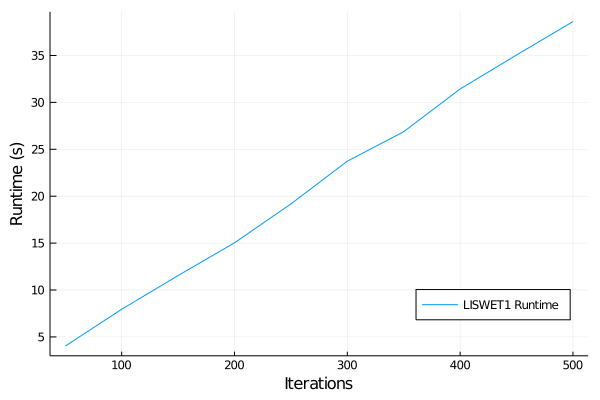
\includegraphics[width=0.8\textwidth]{Plots/LISWET1_iteration_runtime.png}
    \caption{\textit{LISWET1} iteration scaling performance}
    \label{fig:liswet1_iteration}
\end{figure}

\subsubsection{Algorithm Scaling}

One of the requirements of RAM was to illustrate its scaling with number of processors, ideally with a linear relationship. It was expected that any advantage would only be shown in larger tests, and this is shown by the result in Figure \ref{fig:hs21_threading}, where \textit{HS21} shows a broadly linear decrease in performance as more threads are made available to it. As \textit{HS21} has only a single constraint it is not possible to distribute operations over all threads, meaning that additional threads just increase the overhead cost without giving any performance benefit. 

\begin{figure}[tb]
    \centering
    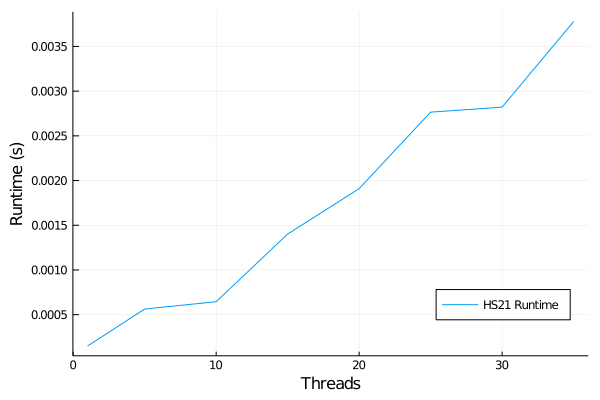
\includegraphics[width=0.8\textwidth]{Plots/HS21 Scaling.png}
    \caption{\textit{HS21} thread scaling performance}
    \label{fig:hs21_threading}
\end{figure}

\begin{figure}[tb]
    \centering
    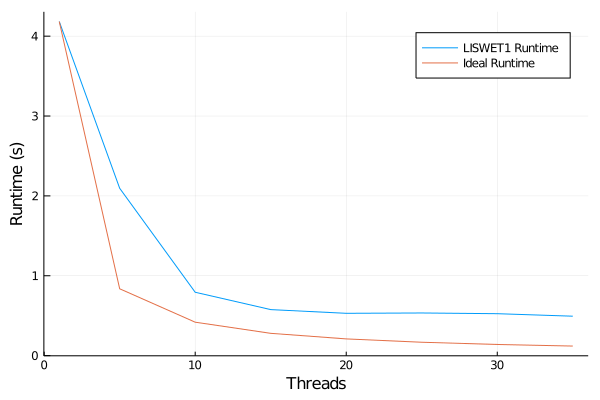
\includegraphics[width=0.8\textwidth]{Plots/LISWET1 Scaling.png}
    \caption{\textit{LISWET1} thread scaling performance}
    \label{fig:liswet1_performance}
\end{figure}

However, when testing larger problems scaling close to the expected result is observed. Figure \ref{fig:liswet1_performance} shows the performance variation as the number of threads is increased for \textit{LISWET1}. Also pictured is the ideal scaling. Putting this on a log-log plot, Figure \ref{fig:liswet1_performance_log}, demonstrates that while additional processors create diminishing returns, good scaling is still present. 

\begin{figure}[tb]
    \centering
    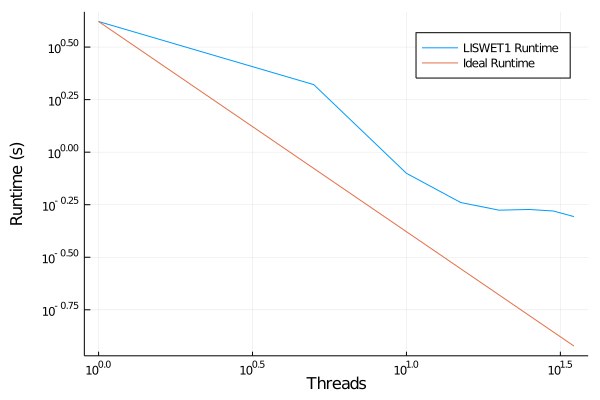
\includegraphics[width=0.8\textwidth]{Plots/LISWET1 log Scaling.png}
    \caption{\textit{LISWET1} thread scaling performance with log scaling}
    \label{fig:liswet1_performance_log}
\end{figure}

The exact cause of the diminishing returns requires further investigation, but it is likely that it is related to overheads with distributing jobs to the threads.

\subsection{DirectSearch.jl}

The comparisons 

%\begin{table}[h] 
%\centering
%\begin{tabular}{llllllll} \toprule
%    {Test}      & \multicolumn{2}{c}{RAM Optimisation}  & {OSQP}   & {IPOPT}    \\ 
%                & 0.1\%                 & 0.01\%                    &          &            \\ \midrule
%    {HS21}      & $8.798\times10^{-5}$  & $8.798\times10^{-2}$      & $1.619\times10^{-3}$ & $1.071\times10^{-2}$\\ 
%    {LISWET1}   & 0.1024                & 0.1256                    & 0.1245   & 3.991      \\ 
%    {LISWET2}   & 0.1151                & 0.1265                    & 0.1239   & 3.433      \\ 
%    {AUG2DC}    & $1.963\times10^{-2}$  & $1.963\times10^{-2}$      & 0.1424   & 1.271      \\ \bottomrule
%\end{tabular}
%    \caption{\label{table:multi_performance}Performance of RAM with 35 Threads (measured in seconds)}
%q\end{table}
\clearpage

%\section{User Guide}\label{section_guide}
This section will give an overview of the main user APIs of both packages, and walkthrough a typical usecase of each. In addition it will go through the process of implementing algorithms within the packages. The information shown here is sourced from the manual pages of the package's documentation. 

As this work is open-source it is hoped that work will be continued on them after the conclusion of the project. For this reason, it is highly likely that the guide shown here will become outdated shortly as the package continues to evolve, therefore the documentaiton for each package should be used as the first reference for its use.

\subsection{RowActionMethods.jl}
\subsubsection{Overview}
\subsubsection{Typical Usage}
\subsubsection{Implementing a Row Action Algorithm}

\subsection{DirectSearch.jl}
\subsubsection{Overview}
\subsubsection{Typical Usage}
\subsubsection{Implementing a Poll Step}
%\clearpage
%
\section{Conclusions and Further Work}\label{sec:conclusion}

\subsection{Evaluation}
The requirements of each of the packages can broadly be divided into two types. The first of these kinds of requirements are those related to performance. Section \ref{sec:testing} illustrated that the performance requirements of the packages have generally been met, with a few caveats. 

For example, the build-times shown when testing \ac{RAM} are incredibly detrimental to the overall utility of the package. However this was expected due to the use of the dual formulation. For Hildreth's algorithm the desired performance, and performance scaling, was demonstrated by the optimisation times. This illustrates that this package, as well as Hildreth's algorithm and row action methods, are useful algorithms for solving difficult quadratic problems, and stack up well against existing algorithms. 

\ac{DS} has also shown that it has met its intended purpose, by implementing the desired algorithms with a good level of performance, while managing to maintain a design that easily allows for algorithms to be modified or added to, without even having to restart a Julia session

\subsection{Future Work}
Throughout the discussion on the design and testing of \ac{RAM} and \ac{DS} several points where designs could be extended or improved have been noted. This section will close the report by giving an overview of the next steps each of the packages can take.

For \ac{RAM}, the first major update that should be made is the addition of constraint modification. This feature was actually present in prototype throughout much of the development of the package, however a late redesign of the storage of the constraints made this incompatible. Including this again, in a manner that allows for problems to not be fully rebuilt would be a strong improvement to the package. 

Additionally for RAM, finding a solution to the problems discussed in \ref{subsub:ram_objective} related to the storage of a sparse factorisation of the problem variable would lead to reduced memory utilisation and improved build times.

For \ac{DS} the improvements to the cache discussed in \ref{sub:ds_cache} would be a very useful addition, possibly integrating the constraint cache into it. The cache would also benefit from memory management tools, limiting the maximum size it can grow to.

Finally, \ac{DS} includes a small section for reporting statistics and information about the solve that it is performing (this was not discussed due to it being in a very basic/prototype form). Formalising the design of this subsection of the program, along with the store/load of configurations (including the cache contents) would greatly benefit the utility of the package.

\subsection{Summary}
\clearpage

\section{Appendix}
\subsection{Acronym Reference}
\begin{acronym}[OrthoMADS]\itemsep10pt
    \acro{RAM}[RAM]{\emph{RowActionMethods.jl}}
    \acro{DS}[DS]{\emph{DirectSearch.jl}}
    \acro{MADS}[MADS]{Mesh Adaptive Direct Search}
    \acro{GPS}[GPS]{General Pattern Search}
    \acro{LTMADS}[LTMADS]{Lower Triangular MADS}
    \acro{OrthoMADS}[OrthoMADS]{Orthogonal MADS}
    \acro{MADS-EB}[MADS-EB]{MADS Extreme Barrier}
    \acro{MADS-PB}[MADS-PB]{MADS Progressive Barrier}
    \acro{MOI}[MOI]{\emph{MathOptInterface.jl}}
    \acro{JuMP}[JuMP]{\emph{Julia for Mathematical Programming}}
    \acro{API}[API]{Application Programming Interface}
    %\acro{LGPL}[LGPL]{Lesser GNU Public License}
\end{acronym}

\subsection{Code Reference}
At the time of submission the code for \textit{RowActionMethods.jl} is available at \url{https://github.com/ImperialCollegeLondon/RowActionMethods.jl/} and the code for \textit{DirectSearch.jl} is available at \url{https://github.com/EdwardStables/DirectSearch.jl}. 

Each package either has or will shortly have documentation and examples of their use.

\clearpage

\bibliographystyle{IEEEtran}
\bibliography{references}

\end{document}